\chapter{Linear Transformations}

The study of linear algebra is really the study of special functions (linear transformations) between vector spaces.  The purpose of this chapter is to extend the notion of functions between numbers to functions between vector spaces using matrices.  We'll see that vector subspaces related to these functions can help us solve many problems we have been looking at in previous chapters.  Thinking about these functions as coming from matrices will help us see the real full power of matrices.

This chapter covers these ideas:

\begin{enumerate}

\item Construct graphical displays of linear transformations.  Graphically explain how to see eigenvalues, eigenvectors, and determinants from these visualizations, as well as when an inverse transformation exists.
\item Know the vocabulary of functions: domain, range, image, inverse image, kernel, injective (one-to-one), surjective (onto), and bijective. 
\item Define linear transformation, and give examples involving both finite and infinite dimensional vector spaces. 
Show that every linear transformation between finite dimensional vector spaces can be represented by a matrix in relation to the standard basis vectors.
\item Describe the column space, null space, and eigenspaces of a matrix. Show that these spaces are vector spaces. 
\item Show that every solution to the linear equation $T(\vec x)=\vec b$ can be written in the form $\vec x = \vec x_p+\vec x_h$, where $\vec x_p$ is a particular solution and $\vec x_h$ is a solution to the homogeneous equation $T(\vec x)=\vec 0$.
\item Explain what it means to compose linear transformations (both algebraically and graphically). Then show how to decompose a matrix as the product of elementary matrices, and use this decomposition (through row reduction) to compute the determinants of large matrices. 


\end{enumerate}


\section{Matrix Transformations}

In this section, we'll explore how matrices transform (reshape, move) the plane and space.  In the next section we will use this geometric idea to define linear transformations.  We'll then show that every matrix represents a linear transformation, and that every linear transformation (between finite dimensional vector spaces) can be represented as a matrix.  The concept that matrices represent functions between vector spaces exposes the real power of matrices.

\subsection{Square Matrices}

Let's start by illustrating how a square matrix $A$ transforms a
vector $\vec x$ by multiplication into another vector $\vec y=A\vec
x$.  For a 2 by 2 matrix such as $A
= \begin{bmatrix}\cl{2\\0}&\cl{1\\3}\end{bmatrix}$, the columns of $A$
tell us what the standard basis vectors $\vec e_1 = (1,0)$ and $\vec
e_2=(0,1)$ get transformed into.  The
product $A\vec e_1 = (2,0)$ is the first column of $A$ and $A \vec e_2
= (1,3)$ is the second column.  Every other vector $(x,y)$ in 2D is
transformed in a similar fashion by considering the product
\begin{align*}
A\begin{bmatrix}x\\y\end{bmatrix} 
&=A\left(x\begin{bmatrix}1\\0\end{bmatrix}+ 
y\begin{bmatrix}0\\1\end{bmatrix}\right) &\text{write $(x,y)$ in terms of
basis $\{\vec e_1, \vec e_2\}$}\\
A\begin{bmatrix}x\\y\end{bmatrix} 
&=A\begin{bmatrix}x\\0\end{bmatrix}+ 
A\begin{bmatrix}0\\y\end{bmatrix} &\text{distribute across addition}\\
&=xA\begin{bmatrix}1\\0\end{bmatrix}+ 
yA\begin{bmatrix}0\\1\end{bmatrix} &\text{pull scalars out front}\\
&=xA\vec e_1+yA\vec e_2.
\end{align*}
From the previous computation, once we know where $(1,0)$ and $(0,1)$ are transformed, we can transform every other vector by just using this information.

This concept of everything depending on $\vec e_1$ and $\vec e_2$ generalizes to any basis.  If $\{\vec b_1, \vec b_2\}$ is a basis for $\RR^2$, then any vector $(x,y)$ can be written as a linear combination of $\vec b_1$ and $\vec b_2$.  By the computation above, once we know what $A\vec b_1$ and $A\vec b_2$ are, we know what $A$ does to any vector $(x,y)$.  Suppose, for example, that $(x,y)=c_1\vec b_1+c_2\vec b_2$.  Then $A(x,y)=A(c_1\vec b_1+c_2\vec b_2)=c_1A\vec b_1+c_2A\vec b_2$.  Everything depends on what $A$ did to the basis vectors $\{\vec b_1, \vec b_2\}$.


We'll illustrate transformations from 2 by 2 matrices with 2D plots (see Figure~\ref{matrix transformation example}). We draw the vectors $(1,0),(0,1)$ and their transformed images $(2,0),(1,3)$.  The unit square transforms into a parallelogram. The matrix transforms a triangle into a new triangle, a circle into an ellipse, and a heart into a slanted heart. One key observation is that the matrix transforms lines to lines, which is why we call the transformation a \emph{linear} transformation.

\begin{figure}
\begin{center}
\begin{tikzpicture}[inner sep=0mm]
\node (middle) {\begin{tabular}{c}
Matrix\\
$\begin{bmatrix}\cl{2\\0}&\cl{1\\3}\end{bmatrix}$\\
Determinant\\
6\\
Eigenvalues\\
2,3\\
Eigenvectors\\
(1,0), (1,1)
\end{tabular}};
\node (B) [left=of middle,xshift=1cm] {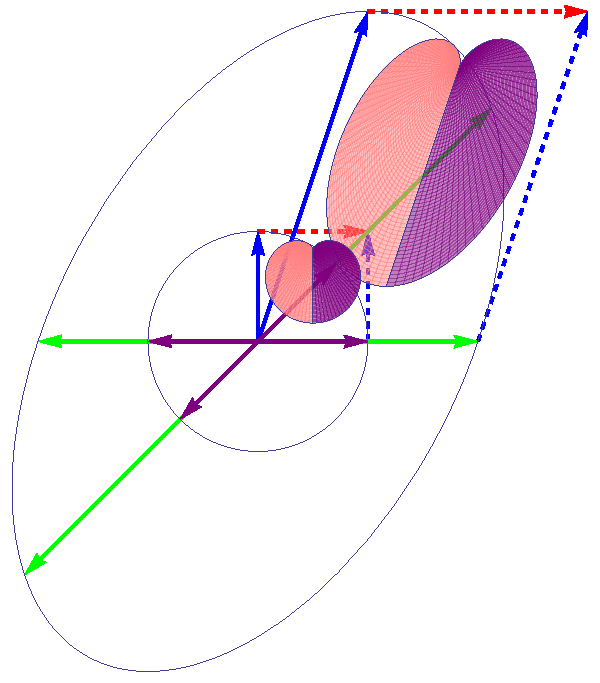
\includegraphics[height=2in]{04-Linear-Transformations/support/LT1b}};
\node (A) [left=of B,xshift=1cm] {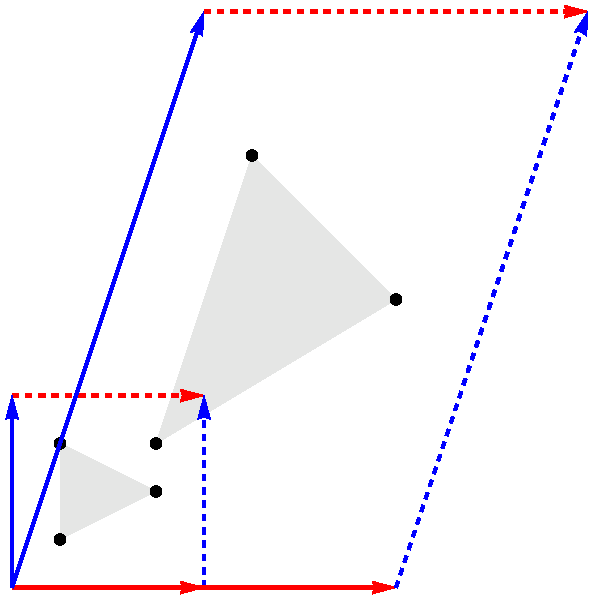
\includegraphics[height=2in]{04-Linear-Transformations/support/LT1}};
\end{tikzpicture}
\end{center}

\caption{{
Two visualizations of a transformation. 
	Matrix transformations map (see left) lines to lines, triangles to triangles, boxes to parallelograms, and (see right) circles to ellipses.		
	Every other point is transformed in a similar fashion (the heart maps to a slanted heart). 
	The determinant measures the increase in area (the parallelogram has 6 times the area of the box, the ellipse has 6 times the area of the circle).	
	Eigenvectors tell you the directions in which the transformation moves points radially outwards. 
	Eigenvalues tell you how much outward stretching occurs in the eigenvector directions. 
}}
\label{matrix transformation example}
\end{figure}

The eigenvectors of the matrix $A$ tell us the directions in which things are transformed radially outwards or inwards ($A\vec x = \lambda \vec x$ means that the vector $\vec x$ is just stretched outward or inward by the factor $\lambda$).  The determinant tells us how much area (or volume for 3 by 3 matrices) is stretched and if the transformation involved a flip.  The determinant is the product of the eigenvalues, so an outward stretch of 2 in one direction followed by an outward stretch of 3 in another direction should result in increasing the area by a factor of $(2)(3)=6$ (see Figure~\ref{matrix transformation example}).  If the determinant of our transformation is zero, then in some direction the transformation squashes things flat, so the area (or volume for 3 by 3 matrices) of the transformed image is zero.

\begin{example}\label{details for four}

Figure \ref{four matrix transformations} illustrates the transformations given by  the four matrices 
$$A = 
\begin{bmatrix}
3&1\\1&3
\end{bmatrix}
,\quad
B = 
\begin{bmatrix}
-1&-1\\-3&1
\end{bmatrix}
,\quad
C = 
\begin{bmatrix}
1&1\\1&-1
\end{bmatrix}
,\quad
D = 
\begin{bmatrix}
1&1\\-1&1
\end{bmatrix}
.$$ 

The matrix $A$ has two positive eigenvalues. The transformation pushes everything outwards.  In the $(1,1)$ directions, lengths are multiplied by 4.  In the $(-1,1)$ direction, lengths are multiplied by 2.  This results in the area increasing by a factor of 8 (i.e., the new area is 8 times the original area).  Notice that the eigenvector directions provide the major and minor axes for the ellipse.  This is always true when the matrix is symmetric.

The matrix $B$ has positive and negative eigenvalues.  The determinant is negative because the image was flipped over in the transformation.  Area is increased by a factor of 4.  The matrix is not symmetric, which is why the eigenvector directions are not the major and minor axes of the transformed ellipse.

We'll look at $C$ and $D$ simultaneously.  The difference between these two matrices is that the columns have been interchanged. Interchanging the columns results in a flip, which causes the determinant to switch signs. Area is doubled for each transformation.  The eigenvalues of $D$ are complex, which means there is no direction in which points are transformed radially outwards---every point is rotated some amount by this transformation.      

\newcommand{\myvfplotheight}{1.8in}
\begin{figure}
\begin{tikzpicture}

\node (symmetric) {\begin{tabular}{c}
Matrix\\
$\begin{bmatrix}\cl{3\\1}&\cl{1\\3}\end{bmatrix}$\\
Determinant\\
8\\
Eigenvalues\\
$4,2$\\
Eigenvectors\\
$(1,1), (-1,1)$
\end{tabular}};
\node [right=of symmetric] {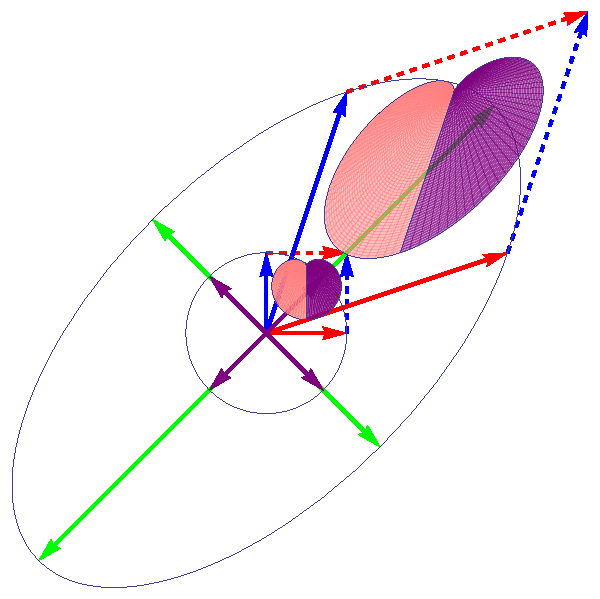
\includegraphics[height=\myvfplotheight]{04-Linear-Transformations/support/LTsymmetricb}};
\node [left=of symmetric] {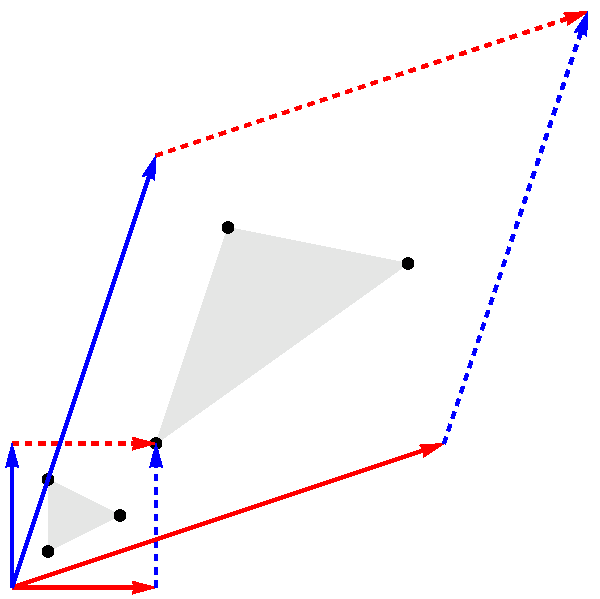
\includegraphics[height=\myvfplotheight]{04-Linear-Transformations/support/LTsymmetrica}};


\node (negative) [below=of symmetric] {\begin{tabular}{c}
Matrix\\
$\begin{bmatrix}\cl{-1\\-3}&\cl{-1\\1}\end{bmatrix}$\\
Determinant\\
-4\\
Eigenvalues\\
$-2,2$\\
Eigenvectors\\
$(1,1), (-1,3)$
\end{tabular}};
\node [right=of negative] {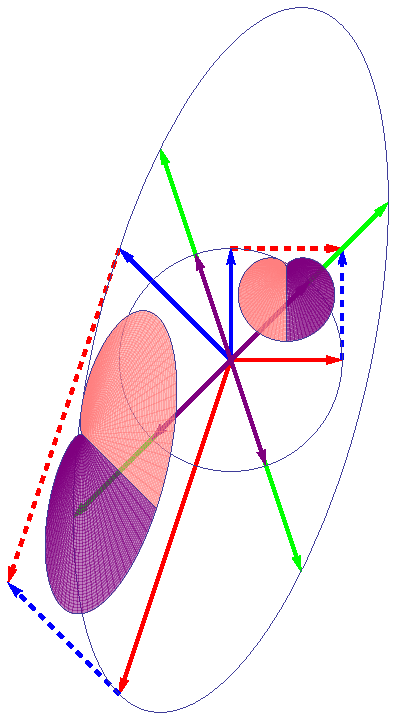
\includegraphics[height=\myvfplotheight]{04-Linear-Transformations/support/LTnegativeb}};
\node [left=of negative] {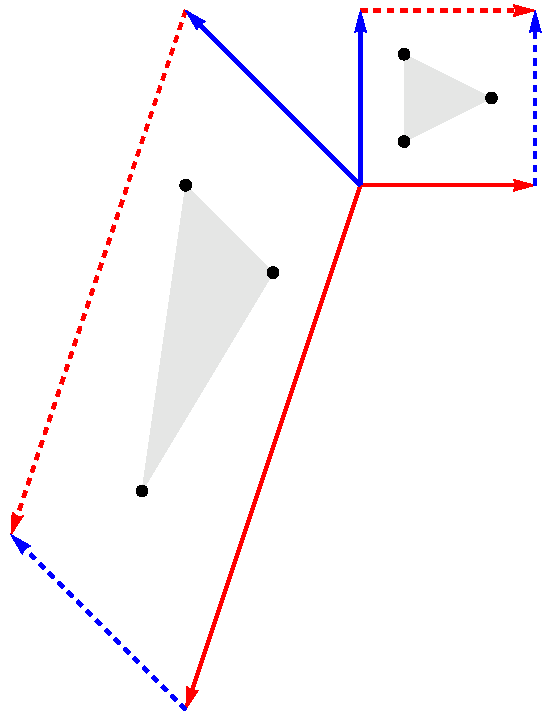
\includegraphics[height=\myvfplotheight]{04-Linear-Transformations/support/LTnegativea}};


\node (irrational) [below=of negative] {\begin{tabular}{c}
Matrix\\
$\begin{bmatrix}\cl{1\\1}&\cl{1\\-1}\end{bmatrix}$\\
Determinant\\
-2\\
Eigenvalues\\
$-\sqrt{2},\sqrt{2}$\\
Eigenvectors\\
$(1-\sqrt2,1), (1+\sqrt2,1)$
\end{tabular}};
\node [right=of irrational] {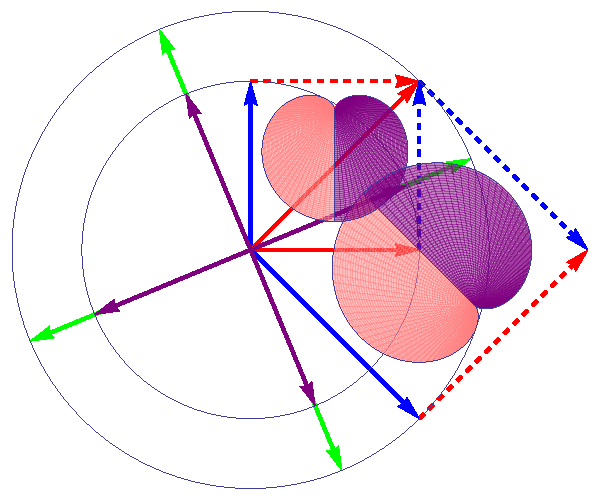
\includegraphics[height=\myvfplotheight]{04-Linear-Transformations/support/LTirrationalb}};
\node [left=of irrational] {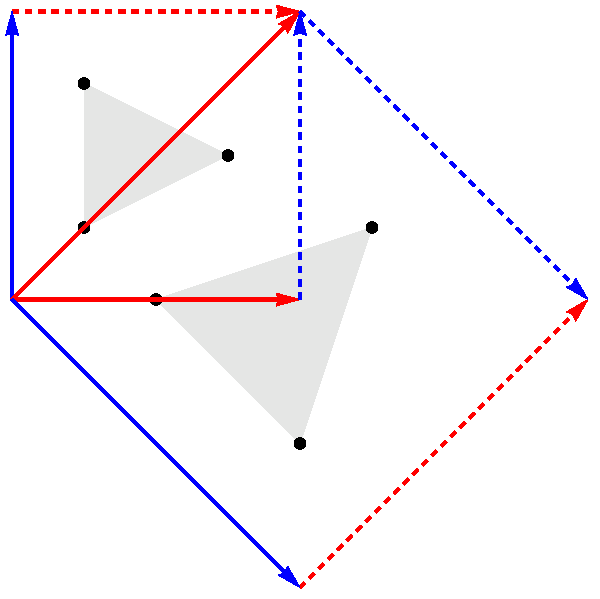
\includegraphics[height=\myvfplotheight]{04-Linear-Transformations/support/LTirrationala}};

\node (complex) [below=of irrational] {\begin{tabular}{c}
Matrix\\
$\begin{bmatrix}\cl{1\\-1}&\cl{1\\1}\end{bmatrix}$\\
Determinant\\
2\\
Eigenvalues\\
$1+i,1-i$\\
Eigenvectors\\
$(-i,1), (i,1)$
\end{tabular}};
\node [right=of complex] {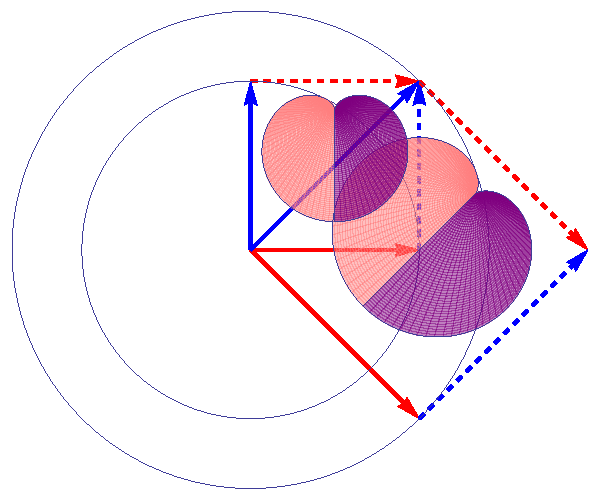
\includegraphics[height=\myvfplotheight]{04-Linear-Transformations/support/LTcomplexb}};
\node [left=of complex] {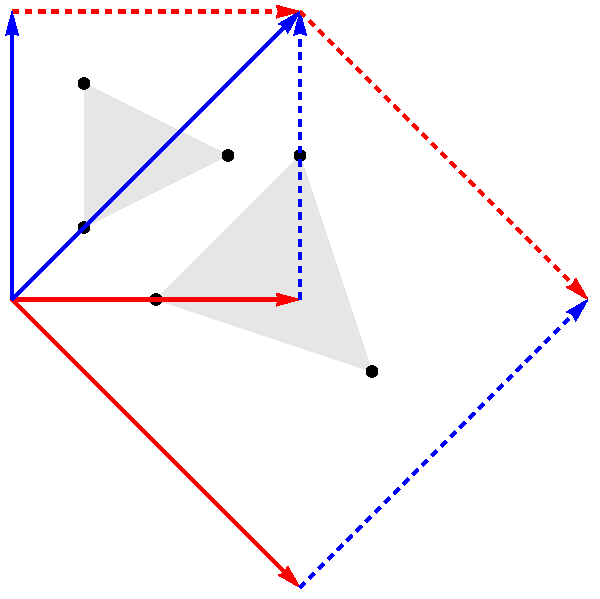
\includegraphics[height=\myvfplotheight]{04-Linear-Transformations/support/LTcomplexa}};

\end{tikzpicture}
\caption{Four 2D transformations. See Example~\ref{details for four} for details. In the pictures on the right, the purple vectors are eigenvectors of length 1, and the green vectors have been scaled by the eigenvalue.
}
\label{four matrix transformations}
\end{figure}
\end{example}

Computers are constantly drawing things in 2D and 3D and they use matrices to transform images to get the pictures and text that you see on the screen.  For this and other reasons, studying and implementing fast matrix multiplication in computers has been a huge field for decades involving millions of dollars and many companies and people.

% \marginpar{PDF documents utilize vector graphics so that you can zoom in on the image as far as you want and still have smooth edges on your text. I have created this text using vector graphics where possible so that you can zoom in on any image and still see a high quality image.} Vector graphics (such as those used in PDF documents) utilize linear transformations to create images.  
% When you zoom in to view a PDF document, the computer redraws all the text so that every corner is still smooth.  
% Scanners and digital cameras store their data as pixels instead of as vectors. 
% If you scan a document and then zoom in, the document appears grainy.  
% Vector graphics prevent pixel errors from occurring as each time you zoom in the computer knows exactly how to transform text so that smooth edges occur. 


\subsubsection{3 by 3 Matrices}

Let's now look at some visualization of 3D transformations. The ideas are similar to what happens in 2D---we just add an additional dimension. This adds another eigenvector direction, and instead of the determinant telling us about a change in area, it now tells us about a change in volume.

\begin{example}\label{3d transformation example}
Figure~\ref{matrix transformation 3d example} illustrates the transformations resulting from the two matrices $\bm{ 2 & 0 & 0 \\ 1 & 2 & 1 \\ 0 & 1 & 2}$
and 
$\bm{ 0 & 0 & -1 \\ 0 & -3 & 0 \\ -2 & 0 & 0}$ in two different ways.  The left images show how the matrices transforms a 3D object.  The right images shows how the matrices transform the unit sphere into an ellipsoid.  The images on the right also include the eigenvector directions. You can log on to Sage to view more images and rotate the images to get a better view of what each transformation does. 

Both matrices have determinant 6, which means that in both cases the volume of objects is multiplied by 6 through the transformation.  The first transformation stretches objects by 1 in the direction $(0,-1,1)$, by 2 in the direction $(-1,0,1)$, and by 3 in the direction $(0,1,1)$.  The second transformation has two directions in which a reflection occurs (the product of two negatives results in a positive determinant).  The amounts of each eigenvalue stretch, together with the eigenvector directions, are listed in the figure.


\begin{figure}
\begin{center}
\begin{tikzpicture}
\node (middle) {\begin{tabular}{c}
Matrix\\
$\bm{ 2 & 0 & 0 \\ 1 & 2 & 1 \\ 0 & 1 & 2}$\\
Determinant\\
6\\
Eigenvalues\\
$1,2,3$\\
Eigenvectors\\
$(0,-1,1)$\\$(-1,0,1)$\\$(0,1,1)$
\end{tabular}};
\node (middle2) [below=of middle] {\begin{tabular}{c}
Matrix\\
$\bm{ 0 & 0 & -1 \\ 0 & -3 & 0 \\ -2 & 0 & 0}$\\
Determinant\\
6\\
Eigenvalues\\
$-3,-\sqrt{2},\sqrt 2$\\
Eigenvectors\\
$(0,1,0)$\\$(\sqrt2/2,0,1)$\\$(-\sqrt2/2,0,1)$
\end{tabular}};
\node  [left=of middle] {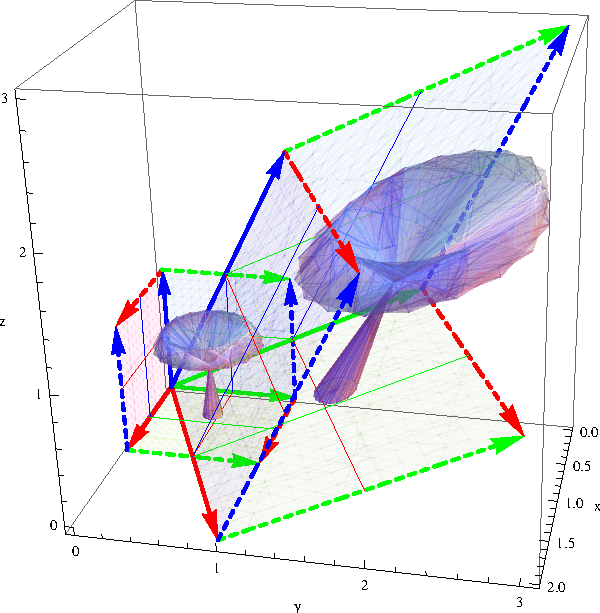
\includegraphics[width=2in]{04-Linear-Transformations/support/LT3da}};
\node  [right=of middle]  {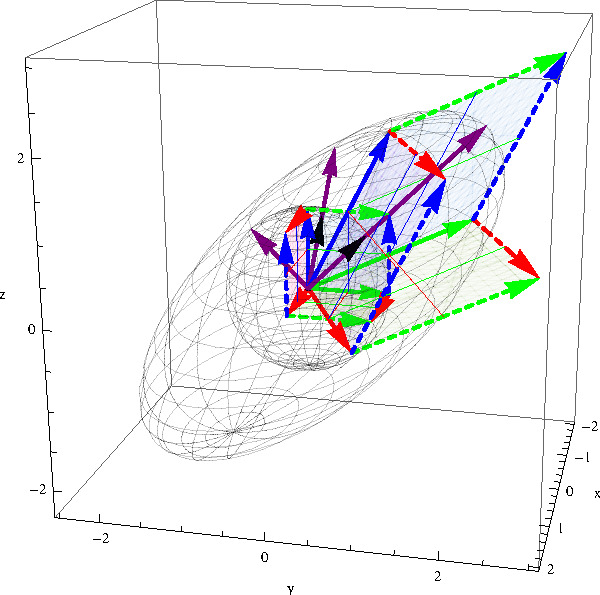
\includegraphics[width=2in]{04-Linear-Transformations/support/LT3db}};
\node  [left=of middle2]{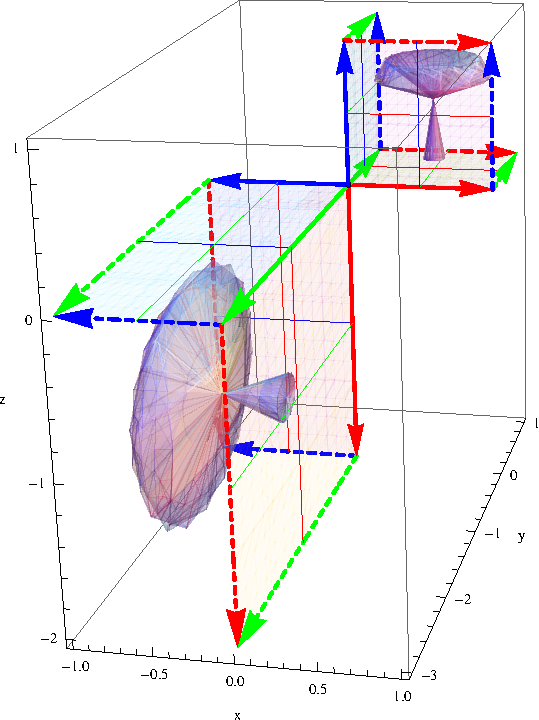
\includegraphics[width=2in]{04-Linear-Transformations/support/LT3d2a}};
\node  [right=of middle2] {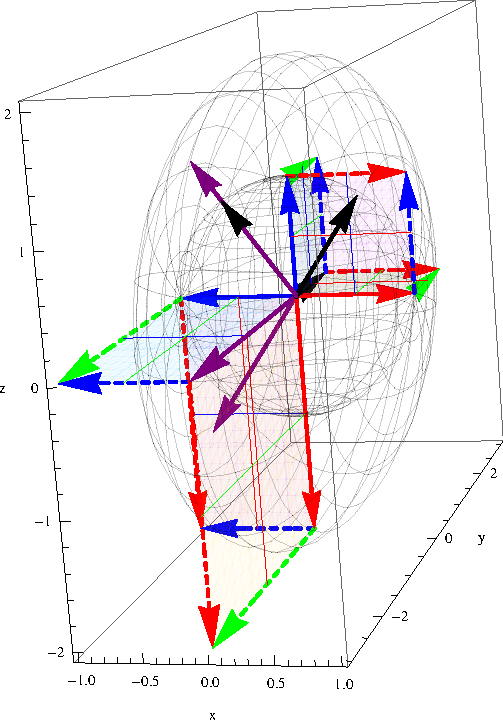
\includegraphics[width=2in]{04-Linear-Transformations/support/LT3d2b}};
\end{tikzpicture}
\end{center}

\caption{{
Two 3D transformations. See Example~\ref{3d transformation example} for details. In the picture on the right, the black vectors are eigenvectors of length 1, where the purple vectors have been scaled by the eigenvalue.}}
\label{matrix transformation 3d example}
\end{figure}
\note{make colors consistent for eigenvectors between the 2d and 3d examples}
\end{example}

\subsubsection{Singular Matrices---Not Invertible}

In all the examples above, we have been looking at square matrices where the determinant is nonzero.  When the determinant is zero, the matrix does not have an inverse and we say the matrix is singular.  This means that the columns are linearly dependent, which means that when we construct a visualization of the transformation, we should see multiple columns overlapping. The next examples illustrate transformations for singular matrices.

\begin{example}
For the matrix 
$A=\bm{1&-2\\-1&2}$, we map $(1,0)$ to $(1,-1)$ and $(0,1)$ to $(-2,2)$. Both vectors lie on the same line.
We obtain the two visualizations below. \marginpar{When the determinant is zero, a 2D transformation takes the entire plane to a line. The column space is the line onto which the transformation maps.}
\begin{center}
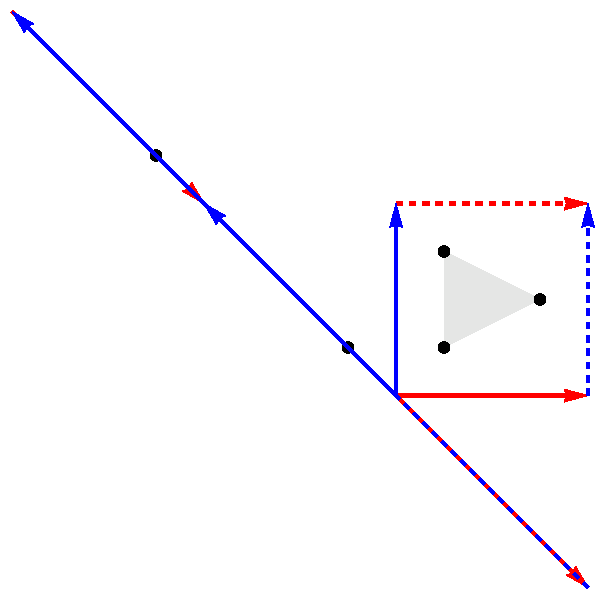
\includegraphics[height=2in]{04-Linear-Transformations/support/LTsingular2da}
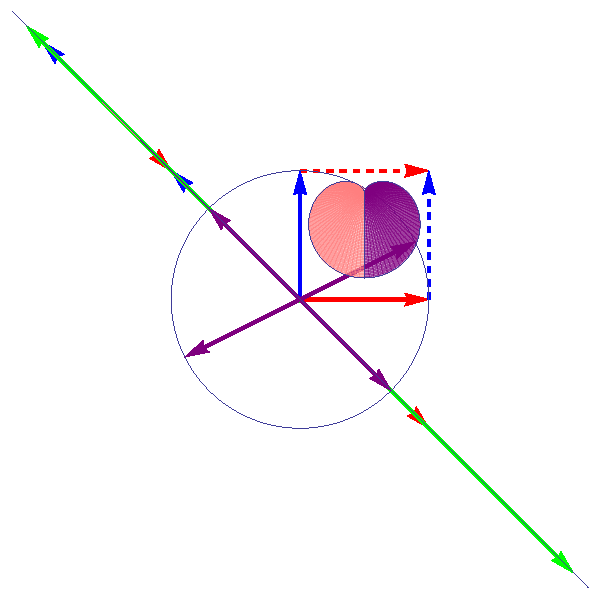
\includegraphics[height=2in]{04-Linear-Transformations/support/LTsingular2db}
\end{center}
Notice that every vector, in addition to $(1,0)$ and $(0,1)$, is mapped onto this same line.  The column space of $A$ is precisely the line given by the span of $(-1,1)$. The column space corresponds directly with the line onto which everything is mapped. Because $\det A = 0$, we know that $\lambda=0$ is an eigenvalue. The corresponding eigenvector $(2,1)$ is drawn in the image on the right. This eigenvector is found by solving $A\vec x = 0$, which means that the set of solutions is the null space. \marginpar{The null space of $A$ is precisely the set of vectors which get squashed to $\vec 0$ by $A$.} Every vector on the line containing $(2,1)$ is transformed to the origin (so in this direction we are squashing an entire line to a point).  Because this transformation squashes two dimension onto a line, it is impossible to invert the transformation (hence no inverse matrix exists).

\end{example}
\begin{example}
For the matrix 
$A=\bm{ 0 & 1 & -1 \\ -1 & 0 & 1 \\ 1 & -1 & 0}$, we map 
the vector $(1,0,0)$ to $(0,-1,1)$, 
the vector $(0,1,0)$ to $(1,0,-1)$, and 
the vector $(0,0,1)$ to $(-1,1,0)$. These three images lie on the same plane (since the determinant is zero).  We obtain two visualizations below. \marginpar{When the determinant is zero, a 3D transformation takes the all of space to a plane (if the rank is 2) or a line (if the rank is 1). The column space is precisely the subspace of $\RR^3$ onto which the transformation squashes things.}
\begin{center}
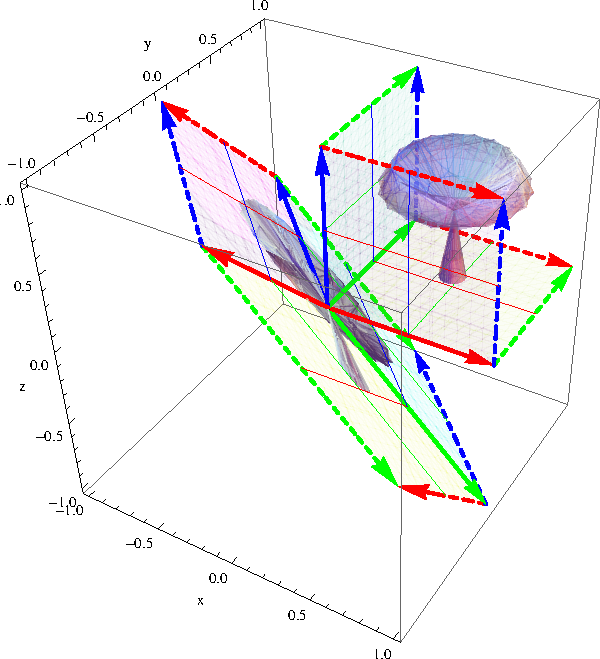
\includegraphics[height=2in]{04-Linear-Transformations/support/LTsingular3da}
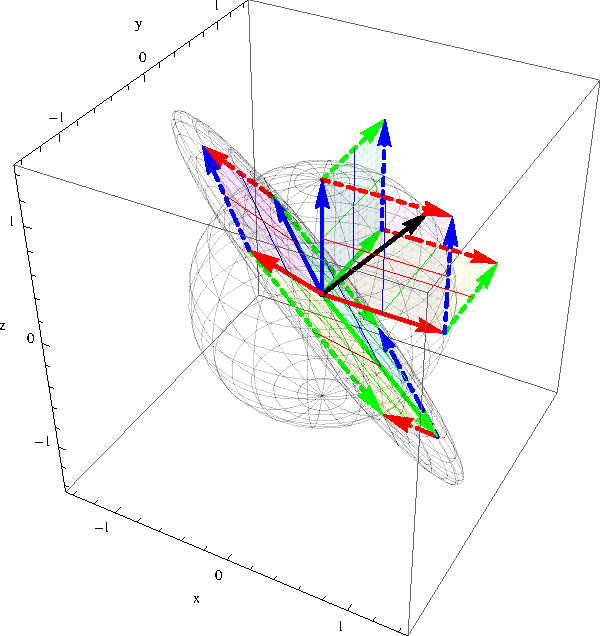
\includegraphics[height=2in]{04-Linear-Transformations/support/LTsingular3db}
\end{center}
Notice that every vector  is mapped onto the same plane containing column vectors of $A$. 
The column space of $A$ is precisely the plane onto which everything is mapped. 
The eigenvector corresponding to $\lambda =0$ is $(1,1,1)$, found by solving $A\vec x=\vec 0$, i.e., finding the null space.
This eigenvector is drawn in the image on the right.  
Anything which lies on the line containing $(1,1,1)$ is also transformed to the origin, so in this direction we are squashing an entire line to a point. 
Because this transformation squashes three dimension onto a 2D plane, it is impossible to invert the transformation (hence $A$ has no inverse). 
Noninvertible square transformations always involve squashing a dimension.

  
\end{example}

In summary, if the determinant is nonzero, then the transformation maps all of 2D to all of 2D, or all of 3D to all of 3D.  If the determinant is zero, then the transformation maps 2D onto a subspace of 2D (a line), or 3D onto a subspace of 3D (a plane or line).  In all cases, the column space of the matrix is precisely the space onto which the transformation maps vectors.

\subsection{Matrices that are not square}

Every example we have looked at in this chapter so far involved either a 2 by 2 or 3 by 3 matrix.  In these cases, we were mapping the plane to the plane, or space to space.  What kind of transformation does a nonsquare matrix represent, and what use would it be?  Any time we see 3D graphics on a computer, or often when we watch television, we are viewing a 3D world that is being presented to us on a 2D plane.  This is an example of a transformation which takes us from 3D to 2D (often written $\RR^3\to \RR^2$).  Projecting a 2D image into 3D (written $\RR^2\to \RR^3$) requires a transformation from 2D to 3D.

The size of the matrix determines the kind of transformation.  For an $m$ by $n$ matrix $A$, the matrix product $A\vec x = \vec b$ requires that $\vec x$ have $n$ components and $\vec b$ have $m$ components.  In other words, the transformation associated with the matrix $A$ takes in vectors in $\RR^n$ and gives back vectors in $\RR^m$.  In notation, the matrix $A_{mn}$ gives us a linear transformation $A_{mn}\colon \RR^n\to \RR^m$.  The number of columns of $A$ is the dimension of the inputs, while the number of rows of $A$ is the dimension of the outputs of the transformation.

Let's look at two more examples.  Then we'll be ready to generalize the patterns we've observed into a general theory about linear transformations.

\begin{example}
Let's look at the two transformations given by the matrices
$A=\bm{0&1\\1&0\\1&1}$ and 
$B=\bm{-2&-1&-1\\1&2&-1}$.
The first transformation requires that we input 2D vectors and returns 3D vectors. To graph this transformation, we notice that multiplying $A$ by the vectors $(1,0)$ and $(0,1)$ returns the two columns of $A$.  So in the $xy$ plane we draw the unit square, and in 3D we graph the parallelogram formed by the two columns.  This is illustrated below. Notice that the unit circle becomes an ellipse in the plane spanned by the columns of $A$.  Again we see that all the output vectors are drawn in the column space of $A$.
\begin{center}
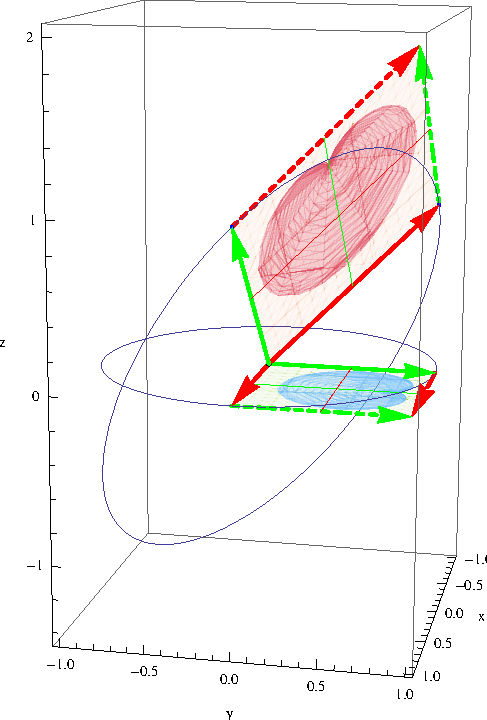
\includegraphics[width=\marginparwidth]{04-Linear-Transformations/support/LT2dto3d}
\end{center}

The transformation given by $B$ requires that we input a 3D vector to obtain a 2D vector.  We graph the unit cube in 3D and graph the columns of $A$ in the $xy$ plane. In this transformation, we are squashing a dimension out of the problem. This is the kind of transformation used to cast shadows in 3D graphics, as well as to present a 2D image of 3D objects for viewing on a screen. 
\begin{center}
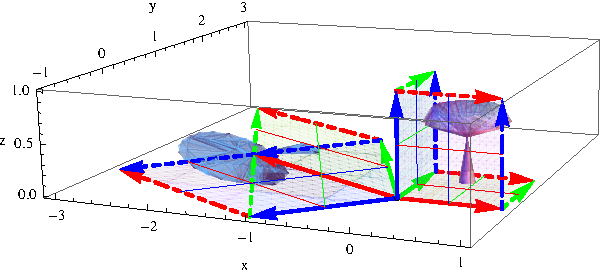
\includegraphics[height=2in]{04-Linear-Transformations/support/LT3dto2d}
\end{center}


\end{example}


\section{What is a Linear Transformation?}
\note{switch the order of the subsections in this section, or even switch the order and then make the general vocabulary a new section.  Here is the email I sent Ben about this:

In keeping with the philosophy that students get lost when lots of definitions and terminology come before concrete examples, I propose reversing the subsections in 4.2 (so it would be "Standard matrix transforms", "Linear Transformations", "General vocabulary of functions"; see my revisions at https://bitbucket.org/jasongrout/linear-algebra/downloads to check the section numbers). This does several things:

1. It puts finding the matrix of a linear transformation just after we've talked about what a matrix does in a linear transformation.  This is very natural (i.e., first is given a matrix, what is the geometry, then given the geometry, what is the matrix?) and very easy to do.

2. Then it is very easy to talk about what a linear transformation is.  For example, after I had the class find a bunch of matrices given the geometry of the transformation, I talked about how f(2,1)=2f(1,0)+f(0,1), and the fact that the linear transformation totally depended on just the values of those two vectors.  This was very natural since they saw obviously that the results of those two vectors gave the entire matrix for a 2 by 2 matrix.  That led naturally into a discussion of linear transformations, the definition, and examples.

3. *then* we formalize the function vocabulary in preparation for talking about the images and kernel of a transformation.  That way the vocabulary comes right before we need it, instead of at the beginning of the chapter, not to be used until the next section.  It also comes after the motivation of linear transformations, inverse matrices, etc. }

\subsection{General Function Notation and Vocabulary}
Let's start with a review of function notation from beginning algebra. 
A function $y=f(x)$ is a rule which assigns to each input $x$ from the domain a value $y$ from the range. 
Notationally we may write $f:D\to R$ to represent the function as a map from $D$ (the domain) to $R$ (the range).  
The sets $D$ and $R$ in previous classes have normally been the set of real numbers. 
Before we proceed to work with functions between vector spaces, we need to build some vocabulary. 
We now consider functions (maps or transformations) from any set $D$ to any set $R$.
\begin{definition}
  \begin{itemize}
  \item Any mapping which assigns to each element of the \define{domain} $D$ exactly one element of the \define{range} $R$ is called a \define{function}. We write $f:D\to R$ to emphasis the domain $D$ and range $R$.  Sometimes the range is called the \define{codomain} of the function.

  \item The \define{image} of an element $x\in D$ is the value $y\in R$ such that $f(x)=y$. We can write $x\mapsto y$ (read ``$x$ maps to $y$'') to illustrate the idea that the input $x$ transforms into the output $y$ through this function.

  \item The \define{image} of $f$, written $\im f=f(D)$, is the set of $y\in R$ which are the image of some $x\in D$.  This means that $\im f$ is always a subset (or is equal to) the range of $f$.  In set notation, we write $$\im f = \{y\in R \st f(x)=y \text{ for some $x\in D$}\}.$$

  \item The \define{preimage} of $y\in R$, written $f^{-1}(y)$, is the set of all $x\in D$ such that $f(x)=y$.  There may be any number of things in $D$ which map to $y$, so the preimage could be any size.
	
  \item We say a function $f$ is \define{one-to-one}, or \define{injective}, if every $y$ value in the image has only one $x$ value which maps to it.  In other words, for every $y\in \im f$, the preimage $f^{-1}(y)$ has one thing in it.  Mathematically, we could also say that if $f(x_1)=f(x_2)$, then $x_1=x_2$.  Another way to say this is that the preimage of any $y\in R$ is always size one or less.

  \item We say a function $f$ is \define{onto}, or \define{surjective}, if $\im f=R$.  In other words, every $y\in R$ is the image of some $x\in D$.  Another way to say this is that the preimage of any $y\in R$ is always size one or more.

  \item We say a function $f$ is \define{bijective} if $f$ is both one-to-one and onto (both injective and surjective).  In other words, every $y\in R$ has exactly one $x\in D$ in its preimage.

  \item If a function $f$ is bijective, we define the \define{inverse} of $f^{-1}\colon R\to D$ to be the function which takes a $y\in R$ and returns the preimage $x\in D$.  This means that $f^{-1}(f(x))=x$, and so $f^{-1}$ inverts $f$.

  \item The composition of two functions $f\colon A\to B$ and $g\colon B\to C$ is a new function $g\circ f\colon A\to C$ that takes an element $a\in A$ and returns the element $c\in C$ given by $c=(g\circ f)(a)=g(f(a))$. Notice that in order to compose two maps, the image of $f$ must be a subset of the domain of $g$.

\end{itemize}
\end{definition}


\begin{example}
Consider the sets $D=\{A,B,C\}$, $R_1=\{1,3,9\}$, and $R_2=\{1,3,7,9\}$.
\begin{enumerate}
	\item Let's define a function $f\colon D\to R_1$ by $f(A)=1$, $f(B)=9$, $f(C)=3$.  The image of $B$ is $9$, so we write $B\mapsto 9$. The image of $f$ is $f(D)=\{1,3,9\}$, so $f$ is onto. The preimage of $3$ is $f^{-1}(3)=C$. This map $f\colon D\to R_1$ is injective and surjective, so it is bijective and has an inverse $f^{-1}$.  The inverse does $f^{-1}(1)=A$, $f^{-1}(9)=B$, and $f^{-1}(3)=C$. 
        \item If we define $f\colon D\to R_2$ by the same rules as above, then $f$ is not surjective (onto) because 7 is not the image of any value in $D$ (i.e., the preimage of $7$ is empty).  You can also see that the function is not surjective since $\im f\neq R_2$.
	\item If we define $f(A)=1$, $f(A)=9$, $f(C)=3$, then $f\colon D\to R_1$ is not a function. There are two things wrong: $f(B)$ is not defined, and $A$ gets mapped to two different values, $A\mapsto 1,9$.
	\item If we define $f\colon D\to R_1$ by $f(A)=1$, $f(B)=3$, $f(C)=3$, then $f$ is a function.  The image of both $B$ and $C$ is $3$ so the preimage of $3$ is $f^{-1}(3)=\{B,C\}$ and has size 2.  This means $f$ is not injective.  Another way to think about this is that $f(B)=f(C)$, but $B\neq C$.
	\item If we define $f\colon D\to R_1$ by $f(A)=1$, $f(B)=3$, $f(C)=9$, and we define $g\colon R_1\to R_2$ by $g(1)=1$, $g(3)=3$, $g(9)=7$, then the composite function $g\circ f$ satisfies $g(f(A))=g(1)=1$, $g(f(B))=g(3)=3$, and $g(f(C))=g(9)=7$. The composite is injective, but not surjective (it misses 9 in $R_2$). 
\end{enumerate}
\end{example}

\subsection{Linear Transformations}
One of the main topics in linear algebra is the study of special types of functions, called linear transformations (or linear mappings) where the domain and codomain (range) are both vector spaces.  All of the transformations resulting from matrices in the first section are linear transformations.  The following definition is a result of noticing the patterns which arose from the examples in the first section.
\begin{definition}[Linear Transformation]
We call a function $T\colon V\to W$ between vector spaces $V$ and $W$ linear function or \define{linear transformation} if both of the following criteria are satisfied:
\begin{enumerate}
	\item $T(\vec v_1+\vec v_2)=T(\vec v_1)+T(\vec v_2)$ for every $\vec v_1,\vec v_2\in V$
	\item $T(c\vec v)=cT(\vec v)$ for every scalar $c$ and vector $\vec v\in V$.
\end{enumerate}
We say that $T$ preserves vector addition and scalar multiplication.  We also say that $T$ preserves linear combinations.
\end{definition}
\marginpar{If $T$ is linear, then the transform of a linear combination is the linear combination of the transforms: $$T\left(\sum_{i=1}^n c_i\vec v_i\right) = \sum_{i=1}^n c_iT(\vec v_i).$$}%
A linear transformation is a function between vector spaces in which you can perform vector addition and scalar multiplication  either before or after applying the function. 
If a function is linear, then repeated application of the definition shows that $$T(c_1\vec v_1+\cdots +c_n\vec v_n) = c_1T(\vec v_1)+\cdots +c_nT(\vec v_n).$$ Linear combinations of vectors becomes linear combinations of the images of each vector when using a linear transformation.  

\marginpar{Once you know what a linear transformation does to a basis, you know what it does to the entire vector space.}%
In particular, this means that if you know the image of each vector in a basis for $V$, you know the image of every vector in $V$, since every vector in $V$ is a linear combination of basis vectors.
\begin{example}
Let's start by illustrating what a linear transformation is not. We'll show that the functions $f(x) = 2x+1$, $g(x)=x^2$, and $h(x,y)=(x+y,xy)$ are not linear transformations.
\begin{enumerate}
\item The function $f(x)=2x+1$ from $\RR$ to $\RR$ (whose graph is a line which does not pass through the origin) is not linear because
  $$f(x+y)=2(x+y)+1 = 2x+2y+1$$ whereas if we transform each point and then sum we obtain $$f(x)+f(y)=2x+1+2y+1 = 2x+2y+2.$$
  Because $f(x+y)\neq f(x)+f(y)$, this function is not linear.
  
  \marginpar{Linear transformations map the $\vec 0$ in the domain to the $\vec 0$ in the range.}%
  Notice that if $T$ is a linear transformation, then $$T(x)=T(0+x)=T(0)+T(x).$$ Thus $T(0)$ must be zero.
 Linear transformations always map the zero vector in the domain to the zero vector in the range.

\item The function $g(x)=x^2$ from $\RR$ to $\RR$ (a parabola) is not linear because 
  $$g(x+y)=(x+y)^2 = x^2+2xy+y^2 = g(x)+g(y)+2xy \neq g(x)+g(y).$$
  Alternatively, we could also look at scalar multiplication to show this function is not linear: $g(2x) = 4x^2$ whereas $2g(x) = 2x^2$, so $g(2x)\neq 2g(x)$.  Raising variables to powers other than 1 results in nonlinear maps.

\item   \marginpar{You can show a function is not linear by providing one example where it violates the conditions in the definition.}%
 The function $h(x,y)=(x+y,xy)$ from $\RR^2$ to $\RR^2$ is not linear. We can show this by looking at an example rather than using variables. We compute $f(1,1)=(2,1)$ and $f(2(1,1)) = f(2,2)=(4,4)$, but $2f(1,1) = (4,2)$.  We have given an example where $f(2\vec x)\neq 2f(\vec x)$, so the map does not always preserve scalar multiplication. 
  The component $xy$ is the problem here. In general, multiplying variables together creates nonlinear functions.  
\end{enumerate}
\end{example}

Now let's look at some examples of linear transformations.  In each example, we will formally show that the function is linear by showing that it preserves both vector addition and scalar multiplication.  The first three examples are crucial, while the last three represent ideas explored more in future classes where vector spaces of infinite dimension are studied.  Many practical applications (like communication, audio and video compression, for example) require knowledge about infinite dimensional vector spaces.  In this class we will focus on linear transformations between finite dimensional vector spaces so that we can represent the transformations using matrices.

\begin{example}
\marginpar{Lines through origin, $f(x)=mx$, are linear transformations from $\RR$ to $\RR$.}%
The function $T(x)=4x$ is linear because
\begin{enumerate}
\item $T(x+y) = 4(x+y) = 4x+4y = T(x)+T(y)$, so $T$ preserves vector addition.
\item $T(cx)=4(cx)=c(4x)=cT(x)$, so $T$ preserves scalar multiplication.
\end{enumerate}
\end{example}

The same reasoning shows that any line through the origin, $y=mx$ for any $m$, is a linear transformation. In the next two examples, we'll show that any function of the form $\vec y = M\vec x$ is a linear transformation as well for any matrix $M$.  \note{The text originally had this sentence here: The reason we use the letter $m$ to represent slope is because the $m$ stands for ``matrix,'' where we replace $x$ and $y$ with vectors.  Is that really true?  Is there a source for this information?} Linear transformations are really just extensions of the simple line $y=mx$ to higher dimensions. The slope becomes a matrix, while the variables become vectors.

\begin{example} \label{ltex matrix1}
The function $T\colon \RR^2\to \RR^2$ defined by $T(x,y)=(2x+3y,x-y)$ is linear.  To show this, we check that $T$ preserves both vector addition and scalar multiplication.
\begin{enumerate}

\item $T((x,y)+(s,t)) = T((x+s,y+t))=(2(x+s)+3(y+t),(x+s)-(y+t)) = (2x+3y,x-y)+ (2s+3t,s-t) = T(x,y)+T(s,t)$, hence the map preserves vector addition.

\item $T(c(x,y))= T(cx,cy) = (2cx+3cy,cx-cy)=c(2x+3y,x-y)=cT(x,y)$, hence the map preserves scalar multiplication.

\end{enumerate}
 We can write this function in matrix form as 
	$$T(x,y)=(2x+3y,x-y)=\begin{bmatrix}2&3\\ 1&-1\end{bmatrix}\begin{bmatrix}x\\y\end{bmatrix}.$$ 	
	\marginpar{The columns of the matrix are the images of the standard basis vectors (1,0) and (0,1). }%
	Notice that $T(1,0)=(2,1)$ is the first column and $T(0,1)=(3,-1)$ is the second column.

\end{example}

\begin{example}\label{ltex matrix2}
Now let's work with a vector space other than $\RR^n$. 
Let $V=P_2(x)$ be the set of polynomials of degree 2 or less, together with the zero polynomial.  
The derivative function $D\colon P_2(x)\to P_2(x)$ defined by $D(a_0+a_1x+a_2x^2)=a_1+2a_2x$ is a linear transformation. 
\begin{enumerate}
	\item The derivative preserves vector addition because $(f+g)'=f'+g'$ by the sum rule for derivatives.
	\item The derivative preserves scalar multiplication becuse $(cf)'=c(f)'$ by the constant multiple rule for derivatives.
\end{enumerate}
The vectors $\{1,x,x^2\}$ are the standard basis vectors for $P_2(x)$. 
Relative to this standard basis, the coordinates of $a_0+a_1x+a_2x^2 = a_0(1,0,0)+a_1(0,1,0)+a_2(0,0,1)$ are just $(a_0,a_1,a_2)$. 
We can then rewrite the derivative transformation in coordinate form as $D(a,b,c) = (b,2c,0)$. 
In matrix form, we write
 $$D(a_0,a_1,a_2)
 =(a_1,2a_2,0)
 =\begin{bmatrix}0&1&0\\0&0&2\\0&0&0\end{bmatrix}\begin{bmatrix}a_0\\a_1\\a_2\end{bmatrix}.$$ 
 Notice that $D(1,0,0)=(0,0,0)$ is the first column, $D(0,1,0)=(1,0,0)$ is the second column, and $D(0,0,1)=(0,2,0)$ is the third column. 
 \marginpar{The columns of our matrix are the coordinates of the images of our basis vectors}
 In general, the columns of our matrix will be the coordinates of the images of the standard basis vectors.
\end{example}

\begin{example}
Let $V=P(x)$ be the set of polynomials, an infinite dimensional vector space with basis $\{1,x,x^2,x^3,\ldots\}$.  
The derivative transformation $D\colon P(x)\to P(x)$ is a linear transformation because of the sum rule and constant multiple rule for derivatives (just as in the last example). 
For those of you who have had calculus 2, Taylor polynomials and Taylor series are all related to this vector space and transformations on it.
\end{example}

\begin{example}
Let $V$ be the set of functions that are infinitely differentiable on the entire real number line (so $e^x$, $\sin x$, $\cos x$, and $x^2$ are in $V$, but $\ln x$, $\sqrt{x}$, and $\tan x$ are not in $V$). 
The derivative transformation $D\colon V\to V$ defined by $D(f) = f'$ is a linear transformation on this space (by the same arguments as the previous example). Notice that you input a function $f$ and get out a function $f'$, so this map takes vectors in $V$ to vectors in $V$.  This space is infinite dimensional, and a basis for this space is so large that we say it is uncountable\footnote{The difference between countably infinite and uncountably infinite is studied in later math classes}.

Let $T\colon V\to \RR$ be the integral transformation, defined by $T(f)=\int_0^1 f(x)dx$.  This transformation takes a function $f$ and returns a real number by integrating over $[0,1]$.  To show this function is linear, we check
\begin{enumerate}
	\item $\ds \int_0^1 f(x)+g(x)dx=\int_0^1 f(x)dx+\int_0^1 g(x)dx$, so $T(f+g)= T(f)+T(g)$ (vector addition is preserved).
	\item $\ds \int_0^1 cf(x)dx =c\int_0^1 f(x)dx$, so $T(cf) = cT(f)$ (scalar multipilcation is preserved).
\end{enumerate}
The derivative and integral are both examples of linear transformations that you have studied before (though you probably didn't use the language of linear transformations on vector spaces!). In real analysis, these ideas are explored in greater depth and become foundational tools for understanding finance, economics, and more.
\end{example}

\begin{example}
Let $V$ be the set of infinitely differentiable functions defined on all of $\RR$.  For any $y(x)$ in $V$, let $$L(y)=y^{\prime\prime}-2xy^\prime+3x^2 y$$ be the differential operator which takes various derivatives of $y$ and combines them together by multiplying by functions of $x$.  This is a linear transformation $L\colon V\to V$ because 
\begin{enumerate}
	\item $L(y_1+y_2)=(y_1+y_2)^{\prime\prime}-2x(y_1+y_2)^\prime+3x^2 (y_1+y_2) = (y_1^{\prime\prime}-2xy_1^\prime+3x^2 y_1) +(y_2^{\prime\prime}-2xy_2^\prime+3x^2 y_2)=L(y_1)+L(y_2)$, so vector addition is preserved.
	\item $T(cy)=(cy)^{\prime\prime}-2x(cy)^\prime+3x^2 (cy) = c(y^{\prime\prime}-2xy^\prime+3x^2 y)=cT(y)$, so scalar multiplication is preserved.
\end{enumerate}
 We use transformations like $L$ to find solutions to differential equations and to show that the set of solutions is a vector space. These ideas are studied more in differential equations, engineering, and physics, and become the foundational tool for understanding mechanical systems, electrical circuits, radio waves, signal processing, and more.  
\end{example}






\subsection{Standard Matrix Representation}
Every matrix $A$ we have studied this semester represents a linear transformation $f(\vec v)=A\vec v$. We can see that the function is linear since
\begin{enumerate}
\item $f(\vec v_1+\vec v_2)=A(\vec v_1+\vec v_2)=A\vec v_1+A\vec v_2=f(\vec v_1)+f(\vec v_2)$, so $f$ preserves vector addition.

\item $f(c\vec v)=A(c\vec v)=c(A\vec v)=cf(\vec v)$, so $f$ preserves scalar multiplication.
\end{enumerate}

Conversely, every linear transformation (between finite dimensional vector spaces) can be expressed in matrix form $T(\vec x)=A\vec x$ for some matrix $A$.  Examples \ref{ltex matrix1} and \ref{ltex matrix2} illustrate how to find the matrix $A$ relative to the standard basis.  To find this matrix, we start by computing the image of each standard basis vector, i.e. $$T(1,0,\ldots,0),\,T(0,1,\ldots,0),\, \ldots,\,T(0,0,\ldots,1).$$ We then place these vectors in the columns of a matrix.  This matrix $A$ is called the standard matrix representation of the linear transformation. We use the word ``standard'' because are using the standard basis vectors to give the coordinates of each vector.  The next two units explore using different basis vectors to describe linear transformations.

\begin{example} Let's find the standard matrix representation of the
  linear transformation $$T(x,y,z,w)=(2x+3y-4z,\,x+y-w,\,z+2x-5w).$$
  We start by computing images of the four standard basis vectors
  \begin{align*}
    T(1,0,0,0)&=(2,1,2), & T(0,1,0,0)&=(3,1,0),\\
    T(0,0,1,0)&=(-4,0,1), & T(0,0,0,1)&=(0,-1,-5).
  \end{align*}
We now place these vectors into the columns of a matrix.  This matrix gives the standard matrix representation of $T$.  We could write $T$ as
$$T(x,y,z,w)=A\vec x=
\begin{bmatrix}
2&3&-4&0\\
1&1&0 &-1\\
2&0&1 &-5
\end{bmatrix}
\begin{bmatrix}
x\\
y\\
z\\
w
\end{bmatrix}.$$ 
The matrix $A$ is called the standard matrix representation of $T$. 
\marginpar{The number of rows is the dimension of the range. The number of columns is the dimension of the domain.}% 
Notice that we input 4D vectors ($A$ has 4 columns) and get out 3D vectors ($A$ has 3 rows).  
\end{example}

Sometimes a linear transformation is described in words.  Examples include things like ``rotate everything 30 degrees'' or ``find the shadow of this object if the sun is located at ...''  In such a case, you can create the standard matrix representation of the transformation by asking where each standard basis vector is sent.  Here is an example.

\begin{example}
Let's rotate an object in the plane counterclockwise by 90 degrees. 
How do we obtain the standard matrix representation of this transformation? 
We find what happens to the standard basis vectors. 
Let $T(x,y)$ be the linear transformation which rotates counterclockwise by 90 degrees.  Then $T(1,0)=(0,1)$ and $T(0,1)=(-1,0)$.  
This means the standard matrix representation of $T$ is 
\begin{align*}
\begin{bmatrix}
\cos \pi/2&\cos\pi\\
\sin\pi/2&\sin\pi
\end{bmatrix}&=\begin{bmatrix}0&-1\\1&0\end{bmatrix} && \text{(a rotation of 90 degrees)}.
\end{align*}

If instead we want to rotate counterclockwise by 30 degrees ($\pi/6$ radians)  then we compute 
$T(1,0) = (\cos \pi/6, \sin \pi/6) = (\sqrt3/2,1/2)$ (the values on the unit circle at $\pi/6$)  and 
$T(0,1) = (\cos 2\pi/3, \sin 2\pi/3) = (-1/2,\sqrt3/2) $ (the values on the unit circle at $\pi/2+\pi/6 = 2\pi/3$). 
This means the standard matrix representation of $T$ is 
\marginpar{
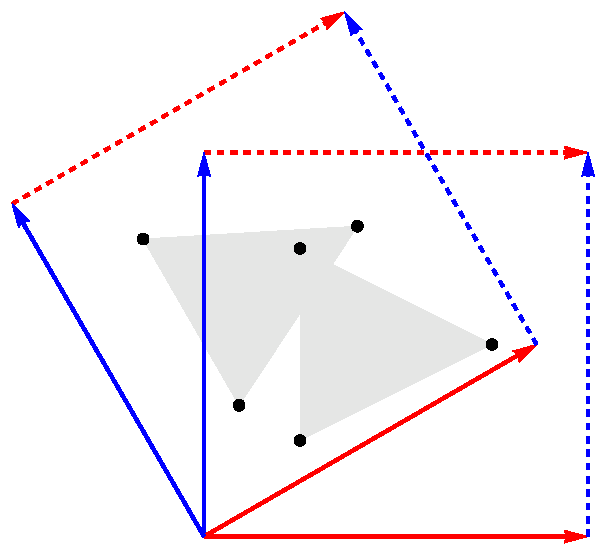
\includegraphics[width=\marginparwidth]{04-Linear-Transformations/support/LTrotate30}

A 30 degree rotation.}
\begin{align*}
\begin{bmatrix}
\cos \pi/6&\cos(\pi/2+\pi/6)\\
\sin\pi/6&\sin(\pi/2+\pi/6)
\end{bmatrix}
&=\begin{bmatrix}\sqrt3/2&-1/2\\1/2&\sqrt3/2\end{bmatrix}  &&\text{(a rotation of 30 degrees)}.
\end{align*}

\end{example}

Let's generalize the pattern we've seen above to rotations through any angle. We can write the image of the second basis vector above in terms of trig function at $\theta$, instead of at $\pi/2+\theta$, if we recall that $\cos(\pi/2+\theta) = -\sin(\theta)$ and $\sin(\pi/2+\theta) = \cos(\theta)$ (these identities just say that shifting cosine left $\pi/2$ gives negative sine, and shifting sine left $\pi/2$ gives cosine).  
We can now write the standard matrix representation of a rotation through $\theta$ degrees as
\begin{align*}
\begin{bmatrix}
\cos \theta&\cos(\pi/2+\theta)\\
\sin \theta&\sin(\pi/2+\theta)
\end{bmatrix}
&=
\begin{bmatrix}
\cos \theta&-\sin\theta\\
\sin \theta&\cos\theta
\end{bmatrix}
&& \text{(a rotation of $\theta$ radians)}.
\end{align*}




Sometimes we are able to extract from a problem information about how a transformation changes vectors other than the standard basis vectors.  When this occurs, provided we know what the transformation does to a basis of the domain, we can still find the standard representation. It just requires a little more work. Let's look at an example. 

\begin{example}
Suppose we know that $T(x,y)$ is a linear transformation from $\RR^2$ to $\RR^3$ and we know that $T(1,1)=(3,0,5)$ and $T(2,0)=(1,-2,0)$. We don't know $A$ yet, but we do know that 
$$
A\begin{bmatrix}1\\1\end{bmatrix} = \begin{bmatrix}3\\0\\5\end{bmatrix} \text{ and }
A\begin{bmatrix}2\\0\end{bmatrix} = \begin{bmatrix}1\\-2\\0\end{bmatrix},\quad \text{ so  } \quad
A\begin{bmatrix}1&2\\1&0\end{bmatrix} = \begin{bmatrix}3&1\\0&-2\\5&0\end{bmatrix}.
$$  
The vectors $(1,1)$ and $(2,0)$ are linearly independent, so they form a basis for $\RR^2$. The matrix formed by placing these vectors in columns, $\begin{bmatrix}1&2\\1&0\end{bmatrix}$, is an invertible matrix since the columns are independent. Since it is invertible, we can multiply both sides of our equation on the right by this inverse to obtain $$A= \begin{bmatrix}3&1\\0&-2\\5&0\end{bmatrix}\begin{bmatrix}1&2\\1&0\end{bmatrix}^{-1} = \begin{bmatrix}3&1\\0&-2\\5&0\end{bmatrix}\begin{bmatrix}0&1\\1/2&-1/2\end{bmatrix} =\begin{bmatrix}1/2&5/2\\-1&1\\0&5\end{bmatrix}.$$ 
We found the standard matrix representation by using the inverse of the matrix of basis vectors that we had. We can check that our matrix $A$ is correct by computing the matrix product 
$$\begin{bmatrix}1/2&5/2\\-1&1\\0&5\end{bmatrix}
\begin{bmatrix}1&2\\1&0\end{bmatrix} 
= \begin{bmatrix}3&1\\0&-2\\5&0\end{bmatrix}$$ to show that $T(1,1)=(3,0,5)$ and $T(2,0)=(1,-2,0)$, as required.  We also know now that $T(1,0) = (1/2,-1,0)$ and $T(0,1)=(5/2,1,5)$, so we know the images of the standard basis vectors. 
\end{example}
 
In general, when you know what a transformation does to any basis of the domain, you can use this to find the standard matrix by multiplying on the right by an inverse.  
Schaum's outlines writes out the equations and then solves them (which is equivalent to using an inverse). In this book, we'll focus on the fact that the inverse matrix is a key tool needed to understand a linear transformation.




  
\section{Subspaces From Linear Transformations}

In the first section where we graphed matrix transformations, we noticed that the column space of the matrix was related to the possible outputs of the transformation. We also saw that the null space of the matrix told us precisely which vectors in the domain were mapped to the origin.  These two spaces associated with matrices are important subspaces related to general linear transformations.  Because a linear transformation could have a domain or range which is infinite dimensional, we need a new word to talk about these subspaces of transformations, even when no matrix exists to represent the transformation.  The new words are image and kernel. Here are the formal definitions.

\begin{definition}
Let $T\colon V\to W$ be a linear transformation.  
\begin{enumerate}
	\item The \define{image} of $T$ (written $\im T$) is the set of all values in $W$ which are the image of some $\vec v$ in $V$. 
	Symbolically we write $$\im T = \{\vec y\in W \ | \ T(\vec x)=\vec y \text{ for some $\vec x\in V$}\}.$$ 
	\item The \define{kernel} of $T$ (written $\ker T$) is the set of all values in $V$ whose image is $\vec 0$ in $W$. 
	Symbolically we write $$\ker T = \{\vec x\in V \ | \ T(\vec x)=\vec 0\}.$$
\end{enumerate}
\end{definition}



If a linear transformation can be represented by a matrix (i.e., when the domain and range have finite dimension), then from the definitions we can see that the image and kernel of the transformation are the same as the column space and null space of the matrix.  Let's formalize this pattern into a theorem.

\begin{theorem}
If $T\colon V\to W$ is a linear transformation between finite dimensional vector spaces and the standard matrix representation of $T$ is $A$, 
\begin{enumerate}
	\item the column space of $A$ is the image of $T$ and 
	\item the null space of $A$ is the kernel of $T$.
\end{enumerate}
\end{theorem}

We already know that the column space and null space of a matrix are vector subspaces.  This is also true of the image and kernel of the transformation.

\begin{theorem}
Let $T\colon V\to W$ be a linear transformation. 
\begin{enumerate}
	\item The image of $T$ is a vector subspace of the range (codomain) $W$. 
	\item The kernel of $T$ is a vector subspace of domain $V$.
\end{enumerate}
\end{theorem}
Notice that the image is a subspace of the range and the kernel is a subspace of the domain. The image is the set of outputs, and the kernel is the set of inputs that map to zero. 

\begin{example}
Let's show that the image of $T$ is a vector subspace of $W$. In the homework, we ask you to show that the kernel is a vector subspace of $V$.  Remember from Theorem~\ref{thm subspace iff closed} that we need to show three things: (1) the zero vector in $W$ is in the image, (2) the image is closed under addition, and (3) the image is closed under scalar multiplication.
\begin{enumerate}
	\item We know that linear transformations map the zero vector in $V$ to the zero vector in $W$.  Thus the image of the zero vector $\vec 0_V$ in $V$ is $T(\vec 0_V) = \vec 0_W$, the zero vector in $W$.  Hence $\vec 0_W$ is in the image.
	\item We need to show that if $\vec y_1$ and $\vec y_2$ are in the image, then so is their sum.  
	Well, since $\vec y_1$ belongs to $W$, we know that $\vec y_1 = T(\vec x_1)$ for some $\vec x_1\in V$.  
	Similarly $\vec y_2 = T(\vec x_2)$ for some $\vec x_2\in V$.  Since $V$ is a vector space, we know that $\vec x_1+\vec x_2$ is also in $V$.
	We can now compute (since $T$ is linear and preserves addition) \marginpar{Linear transformations preserve addition. This is why the image is closed under addition.}  $$T(\vec x_1+\vec x_2) = T(\vec x_1)+T(\vec x_2) = \vec y_1+\vec y_2$$ 
	which means that the sum $\vec y_1+\vec y_2$ is the image of $\vec x_1+\vec x_2$. 
	This shows that the image is closed under vector addition.
	\item The only thing that remains is to show that if $\vec y$ is in $W$, then so is any scalar multiple of $\vec y$. Since $\vec y\in W$, we know there is some $\vec x\in V$ such that $T(\vec x)=\vec y$. Since $V$ is a vector space, we know that $c\vec x$ is also in $V$ for any $c$.  Now we can compute (since $T$ is linear and preserves scalar multiplication) 
	\marginpar{Linear transformations preserve scalar multiplication. This is why the image is closed under scalar multiplication.}
	$$T(c\vec x) = cT(\vec x) = c\vec y$$ which means that $c\vec y$ is the image of $c\vec x$.
	This shows that the image is closed under scalar multiplication.
	
\end{enumerate}

Your job in the homework will be to show that the kernel of a linear transformation is a vector subspace of the domain $V$.

\end{example}

Now that we know the image and kernel of a transformation are vector subspaces, we can look for spanning sets, bases, and find the dimensions of these spaces. We used the word ``rank'' for the dimension of the column space, but have not yet given a name to the dimension of the null space.  Here are some more definitions.

\begin{definition} 
Let $T\colon V\to W$ be a linear transformation. 
The dimension of the image of $T$ is called the \define[rank!linear transformation]{rank} of $T$ (just as the rank is the dimension of the column space).
The dimension of the kernel of $T$ is called the \define{nullity} of $T$.  Similarly, the \define{nullity} of a matrix is the dimension of the null space of the matrix.
\end{definition}

Now that we have some words to describe the dimensions of the image and kernel, we can state one of the key theorems which relates these two subspaces.  A basis for the column space of a matrix $A$ is simply the pivot columns of $A$. We find a basis for the null space by solving for all the variables in terms of the free variables, which means that each free variable contributes a vector to the basis of the null space.  Since the free variables correspond to nonpivot columns, and the column space corresponds to pivot columns, we see that the sum of the dimensions of the column space and null space must always equal the number of columns.  

\begin{theorem}[The Rank-Nullity Theorem]
Let $T\colon V\to W$ be a linear transformation between finite dimensional vector spaces, whose standard matrix representation is $A$.  Then 
\begin{enumerate}
	\item The rank of $T$ is the number of pivot columns of $A$. 
	\item The nullity of $T$ is the number of nonpivot columns of $A$. 
	\item The rank of $T$ plus the nullity of $T$ is always equal to the dimension of $V$. 
\end{enumerate}
\end{theorem}
Notice that the third item does not refer at all to the matrix $A$.  The third fact only relies on $V$ having finite dimension.  Even though our reasoning above only proves it is true when $W$ also has finite dimension, it is still true even if $W$ has infinite dimension (in which case $T$ does not have a standard matrix representation). 


\begin{example}
Consider the linear transformation $T\colon {\RR}^5\to {\RR}^6$ with standard matrix 
$$A=\begin{bmatrix}
 1 & 2 & 0 & 1 & 1 \\
 2 & -3 & -7 & -1 & 13 \\
 0 & 1 & 1 & 1 & -1 \\
 4 & 0 & -8 & 4 & 20 \\
 3 & 0 & -6 & 3 & 15 \\
 0 & 0 & 0 & 0 & 0
 \end{bmatrix} 
\xrightarrow{rref}
\begin{bmatrix}
 1 & 0 & -2 & 0 & 4 \\
 0 & 1 & 1 & 0 & -2 \\
 0 & 0 & 0 & 1 & 1 \\
 0 & 0 & 0 & 0 & 0 \\
 0 & 0 & 0 & 0 & 0 \\
 0 & 0 & 0 & 0 & 0
\end{bmatrix}.$$

The column space of $A$ is the span of the columns of $A$. 
The image $T$ is all vectors of the form $A\vec x$, which is also the span of the columns of $A$. 
This means that the column space of $A$ and the image of $T$ are the same vector subspace of the range of $T$, ${\RR}^6$.
A basis for this vector subspace is the set of pivot columns $$\{(1, 2, 0, 4, 3, 0),\, (2, -3, 1, 0, 0, 0),\, (1, -1, 1, 4, 3, 0)\},$$ so the column space has dimension 3. The ranks of both $A$ and $T$ are 3.

To find the null space of $A$, and hence the kernel of $T$, we solve the equation $A\vec x=0$.  The 3rd and 5th columns correspond to the free variables.  We can write the solution as 
$$
\begin{matrix}
x_1-2x_3+4x_5=0\\
x_2+1x_3-2x_5=0\\
x_3=x_3\\
x_4+x_5=0\\
x_5=x_5
\end{matrix}
\Rightarrow
\begin{matrix}
x_1=2x_3-4x_5\\
x_2=-1x_3+2x_5\\
x_3=x_3\\
x_4=-x_5\\
x_5=x_5
\end{matrix}
\Rightarrow
\begin{bmatrix}
x_1\\
x_2\\
x_3\\
x_4\\
x_5
\end{bmatrix}=
x_3
\begin{bmatrix}
2\\
-1\\
1\\
0\\
0
\end{bmatrix}+
x_5
\begin{bmatrix}
-4\\
2\\
0\\
-1\\
1
\end{bmatrix}.
$$
We see that the null space is the span of the vectors $$\{(2,-1,1,0,0),\,(-4,2,0,-1,1)\}.$$ 
The kernel of $T$ is a vector subspace of the domain of $T$, ${\RR}^5$.
The numbers in these vectors are the negatives of the numbers in the nonpivot columns of rref, with a 1 or 0 placed in the spots representing the free variables.  
The reason we negate all the numbers is that we have to subtract these numbers from both sides of the first equation to solve for each variable in terms of the the free variables.  
The nullity of $T$ is 2 (the number of free variables). 
The rank plus the nullity equals $3+2=5$, the dimension of the domain (or number of columns).
\end{example}

\section{Applications of the kernel}




\subsection{Solutions to Systems and the Kernel}

The kernel arises from solving the equation $T(\vec x)=\vec 0$.  Can we use the kernel to help us solve the equation $T(\vec x)=\vec b$?  The answer is amazingly yes. The key lies in the fact that if both $\vec x_1$ and $\vec x_2$ are solutions to $T(\vec x)=\vec b$, then $$T(\vec x_1-\vec x_2)=T(\vec x_1)-T(\vec x_2)=\vec b - \vec b=\vec 0,$$
so $x_1-x_2$ is in the kernel of $T$ (did you see how we used the properties from $T$ being a linear transformation?).  Solving for $\vec x_1$ gives us the fact that $\vec x_1=\vec x_2+\vec x_h$ where $\vec x_h$ is some vector in the kernel of $T$. On the other hand, if $\vec x_h$ is any vector in the kernel, then $$T(\vec x_1+\vec x_h)=T(\vec x_1)+T(\vec x_h)=\vec b + \vec 0=\vec b,$$
so adding any vector in the kernel of $T$ to $\vec x_1$ gives anothers solution to $T(\vec x)=\vec b$.  Let's formalize this into a theorem.
\begin{theorem}
Let $T$ be a linear transformation. Consider the nonhomogeneous equation $T(\vec x)=\vec b$.
If $\vec x_p$ is one particular solution to the equation $T(\vec x)=\vec b$ (i.e., $T(\vec x_p)=\vec b$), then every solution can be written in the form $\vec x = \vec x_p+\vec x_h$, where $\vec x_h$ is a solution to the corresponding homogeneous equation $T(\vec x)=\vec 0$.  In other words, every solution to the nonhomogeneous equation is found by first finding a particular solution $\vec x_p$ and then adding $\vec x_p$ to every vector in the kernel.  
\end{theorem} 
This theorem is a key tool used to solve differential equations.  Once you know one solution, you can find every other solution by just adding the solution to every vector in the entire kernel. This makes the kernel an extremely useful subspace to understand.

\begin{example}
Suppose that a system of equations gives rise to the augmented rref matrix on the left below.  Then the solution is on the right.

\begin{align*}
\begin{bmatrix}[ccccc|c] 0&1&0&2&0&0\\0&0&1&3&0&1\\0&0&0&0&1&4\\0&0&0&0&0&0\end{bmatrix}
\longrightarrow
\begin{bmatrix}x_1\\x_2\\x_3\\x_4\\x_5\end{bmatrix} 
= \begin{bmatrix}0\\0\\1\\0\\4\end{bmatrix}
+x_1\begin{bmatrix}1\\0\\0\\0\\0\end{bmatrix}
+x_4\begin{bmatrix}0\\-2\\-3\\1\\0\end{bmatrix}  
\end{align*}
A particular solution to this system is $\vec x_p=(0,0,1,0,4)$ (obtained by letting the free variables $x_1$ and $x_4$ both be zero).  The null space is the span of the vectors $(1,0,0,0,0)$ and $(0,-2,-3,1,0)$. Notice that every solution to the system can be written in the form $\vec x_p +\vec x_h$, where $\vec x_h$ is a vector in the null space.
\end{example}
 
\subsection{Eigenspaces are Null Spaces}
We have already noticed in the first section that the eigenvectors of a matrix tell us the directions in which a transformation pushes points radially outwards or inwards.  These directions provide us a line (vector subspace) in which all transforming is done radially outwards (or inwards if the eigenvalues are less than one in magnitude).  Recall that corresponding to each eigenvalue is an infinite collection of eigenvectors. By definition, the zero vector is not an eigenvector, hence the set of eigenvectors cannot be a vector subspace.  However, if we include the zero vector, we obtain a vector space. We now make some formal definitions.

\begin{definition}[Eigenspaces]
If $\lambda$ is an eigenvalue of a matrix $A$, then the set of vectors $E_\lambda = \{\vec x \st A\vec x = \lambda \vec x\}$ (the eigenvectors together with zero) is called the eigenspace of $A$ corresponding to $\lambda$. 

We say that $\lambda$ is an eigenvalue of a linear transformation $T\colon V\to V$ (notice the domain and range are the same) if 
$T(\vec x)=\lambda \vec x$ for some nonzero $\vec x$, called an eigenvector of $T$ corresponding to $\lambda$. 
If $\lambda$ is an eigenvalue of $T$, then the set of vectors $E_\lambda = \{\vec x \st T(\vec x) = \lambda \vec x\}$ (the eigenvectors together with zero) is called the eigenspace of $T$ corresponding to $\lambda$. 
\end{definition}
We find eigenvectors of a matrix by solving $(A-\lambda I)\vec x = \vec 0$ which means that the eigenspace $E_\lambda$ is precisely the null space of $(A-\lambda I)$.  Because the eigenspace is a null space, we know that it is a vector space.

%Another important subspace which occurs when considering a square matrix is the eigenspace of an eigenvector.  If we pick a single eigenvalue $\lambda$ and add $\vec 0$ to the set of eigenvectors, then this space is a subspace of the domain. This is because if $\vec x_1$ and $\vec x_2$ are both eigenvectors, then $A(\vec x_1+\vec x_2) = A\vec x_1+A\vec x_2 = \lambda\vec x_1+\lambda\vec x_2 = \lambda(\vec x_1+\vec x_2)$, which means $\vec x_1+\vec x_2$ is an eigenvector as well.  Similarly, $A(c\vec x_1) = c(\lambda\vec x_1)=\lambda (c\vec x_1)$, which means $c\vec x_1$ is an eigenvector as well. This shows that each eigenspace of $A$ (one for each eigenvalue) is a vector subspace of the domain. Any vector in this eigenspace will be transformed radially from the origin when you draw the transformation.  If the eigenvalue is zero, then the eigenspace will be part of the null space.


\subsection{Squashing in transformations}

The dimension of the kernel of a linear transformation can help us understand how much squashing goes on in the transformation.  If the kernel is trivial (only the zero vector), then no vectors will be mapped to zero except for zero itself.  This means that the transformation will map lines to line, planes to planes, 3D volumes to 3D volumes, etc.  In this case, we say the linear transformation is nonsingular. If the domain and range have the same dimension, then the transformation will have an inverse. 

However, if the transformation has a nontrivial kernel (i.e., not just the zero vector), then the dimension is squashed in some direction. We call the transformation singular, and it cannot have an inverse. For example, an entire line could be mapped to a point, or an entire plane could be mapped to a line.  


\subsection{Casting Shadows using the Null Space}

The null space of a matrix tells us the directions which get mapped to zero under the linear transformation corresponding to the matrix.  We know how to compute the null space if we are given a matrix.  What if we are given the null space and asked for a matrix with that null space?  Can we find a matrix with a specific null space?  Let's explore this issue by figuring out a linear transformation that tells how shadows are cast on the ground.

When the sun shines down on you during the afternoon, it casts a shadow on the ground.  The function which takes a point $(a,b,c)$ and gives back the $(x,y)$ coordinate of the shadow is a linear transformation (notice that straight things cast straight shadows!).  Suppose you are positioned at the origin standing with your head pointing up along the $z$ axis.  Imagine putting a stick at your feet pointed directly at the the sun (so it casts no shadow).  This stick gives a vector that points directly at the sun.  Any object along that direction (between your feet and the sun) will cast a shadow at your feet.   Since anything along the line between your feet at the origin and the sun casts a shadow at your feet, that entire line is the null space of our linear transformation (i.e., all of those vectors get mapped to $(0,0)$).  Can we find a matrix for this shadowy linear transformation?  That will let us calculate the shadow of any object.

Since points already on the ground do not cast a shadow, we know that the vector $(x,y,0)$ gets mapped to $(x,y)$.  In particular, $(1,0,0)\mapsto (1,0)$ and $(0,1,0)\mapsto (0,1)$.  As discussed above, we also know that a vector pointing directly at the sun gets mapped to $(0,0)$.

\begin{example}
Suppose that the sun is positioned on a line containing the vector $(2,1,4)$ (i.e., the stick at your feet pointing at the sun is the vector $\vec v=(2,1,4)$).
We want transformation that has this vector as a basis for the kernel.  
Because we're mapping from 3D onto the $xy$ plane, we need a $2$ by $3$ matrix. 
Divide every component in $\vec v$ by $4$ to get a 1 in the $z$ component. The vector $(1/2,1/4,1)$ looks a lot like the vectors we obtain by having a free variable $z$.  The null space is all linear combinations of this vector, which we can express as $$\bm{x\\y\\z} = z\bm{1/2\\1/4\\1}. $$ We now have two equations: $x=1/2 z$ and $y=1/4z$, or $x-\frac12 z=0$ and $y-\frac14 z=0$.  Now we just write down the matrix associated with this system of linear equations: $$A=\bm{1&0&-1/2\\0&1&-1/4}.$$
\marginpar{
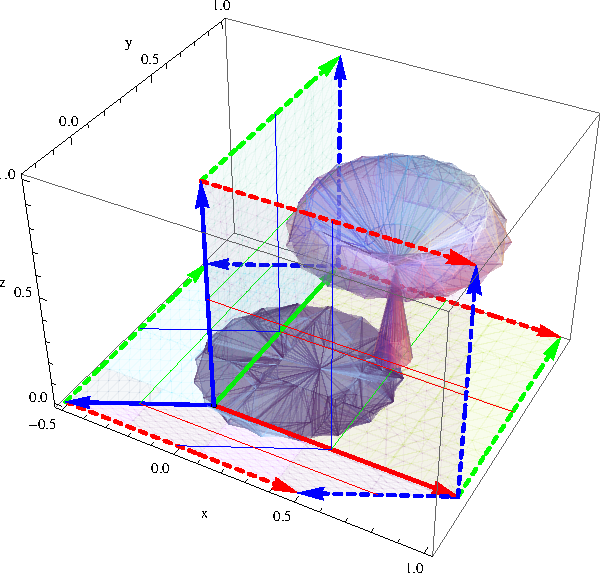
\includegraphics[width=\marginparwidth]{04-Linear-Transformations/support/LTshadow}

Knowing the null space is sufficient to find a transformation to cast shadows onto the $xy$ plane.
}
Notice that since made sure that the left two columns formed an identity matrix, we get the other mappings that we wanted: $(1,0,0)\mapsto (1,0)$ and $(0,1,0)\mapsto (0,1)$.
The image in the margin illustrates this projection. 
\end{example}


\section{Composition of Linear Transformations}
The composition of two functions $f$ and $g$ is a new function $(g\circ f)(x)$ defined by $(g\circ f)(x) = g(f(x))$.  The idea is that you input an $x$ value into $f$, and then input $f(x)$ into $g$.  The same principle applies to linear transformations.  If $S\colon U\to V$ and $T\colon V\to W$ are two linear transformations, then the composition $T\circ S\colon U\to W$ is defined by $T(S(\vec u))$ (where $S(\vec u)$ is a vector in $V$ which serves as an input to $T$). Let's look at an application of function composition. 

\begin{example}
If we want to rotate an object 90 degrees counterclockwise, and then mirror-image the object about the $y$-axis, we can achieve this by composing two linear transformations. \marginpar{When multiple linear transformations are involved, we often use the notation $S_A$ or $T_A$ to represent the standard matrix representations.}%
The linear transformation $S$ which rotates and object in the plane 90 degrees has standard matrix representation $S_A = \bm{0&-1\\1&0}$, since $S(1,0) = (0,1)$ and $S(0,1)=(-1,0)$.  
The linear transformation $T$ which flips objects about the $y$ axis has standard matrix representation $T_A = \bm{1&0\\0&-1}$, since $T(1,0)=(1,0)$ and $T(0,1)=(0,-1)$.  The composition $T(S(x,y))$ will first perform the rotation $S(x,y)$ and then reflect the result about the $y$ axis. We compute $S(T(x,y))$ by computing 
\begin{align*}
  (S\circ T)(x,y)&=S_A\left(T_A\bm{x\\y}\right) = \bm{1&0\\0&-1}\left(\bm{0&-1\\1&0}\bm{x\\y}\right) \\
  &= \bm{1&0\\0&-1}\bm{0&-1\\1&0}\bm{x\\y}\\
  &=\bm{0&-1\\-1&0}\bm{x\\y}.
\end{align*}
Notice that function composition is precisely matrix multiplication.
\end{example}


The composition of two linear transformations has as its standard matrix representation the product of the standard matrix representations of each transformation. 
In other words, if $S\colon  U\to V$ and $T\colon V\to W$ are both linear transformations with standard matrices $S_A$ and $T_A$, then $T\circ S\colon U \to V$ (sometimes just written $TS$) has standard matrix $(TS)_A=T_AS_A$. 
Notice that in order for this composition to make sense, the range of $S$ and domain of $T$ must match, which means that the number of rows of $S_A$ must equal the number of columns of $T_A$ (in other words you have to be able to compute the matrix product $T_AS_A$). 
One of the primary purposes for matrix multiplication is to compose linear transformations.\note{originally, this was the text: Matrix multiplication was purposefully created so that the product of matrices equals the composition of linear transformations.  Citation needed?} 

When the domain and range of a linear transformation have the same dimension, the standard matrix is a square matrix.  
In such cases, we can compute the determinant of a transformation, find the eigenvalues and eigenvectors of a transformation, and ask if the transformation is invertible. 
If the transformation $T$ is invertible with standard matrix $A$, then the standard matrix of the inverse is $A^{-1}$. Symbolically we write $T^{-1}(\vec x) = A^{-1}\vec x$. 


\section{Elementary Matrices and Determinants}

% In the patterns chapter, Theorem~\ref{thm det product} stated that $|AB|=|A||B|$. The determinant of a linear transformation measures how much the transformation ``stretches'' space. If one transformation $S$ stretches space by 2 units, and another transformation $T$ stretches space by $3$ units, then applying the first transformation followed by the second should stretch space by $2\cdot 3=6$ units. In other words, the product of the determinants of linear transformations is should be the determinant of the composition of the linear transformations. This is a geometric reason as to why $|AB|=|A||B|$. 

To quickly understand a complicated linear transformation or complicated matrix, it is often easiest to break the transformation down into a series of very simple transformations, or break the complicated matrix down into a product of much simpler matrices.  Understanding each part because easy, and then combining what you know about the parts tells you things about the complicated transformation or structure.  In this section, we will examine one way to break a matrix up into a product of much simpler matrices that leads us to a very fast method used in industry to calculate the determinant, solve systems of equations, and much more.

The goal here is to factor the matrix $A$ into the product of so-called ``elementary matrices,'' which are simple matrices directly related to row reduction.  Whenever we write down a product of matrices, we are also writing down a composition of linear transformations, so we are also exploring how to make a take apart a complicated linear transformation into a series of much simpler ones.

\begin{definition}
An \define{elementary matrix} is a matrix obtained by performing one of the following row operations to the identity matrix.
\begin{enumerate}
	\item Switch any two rows.
	\item Multiply a row by a nonzero constant.
	\item Add a multiple of one row to another.
\end{enumerate}
\end{definition}
The row operations above are precisely the operations we use to perform Gaussian elimination. 
You can also undo each row operation above:
\begin{enumerate}
	\item The inverse of switching two rows is to switch the same rows again.  
	\item The inverse of multiply a row by $k$ is to multiply the same row by $1/k$.  
	\item The inverse of adding $k$ times row $i$ to row $j$ is to subtract $k$ times row $i$ from row $j$. 
\end{enumerate}
Three examples of elementary matrices follow, along with their inverses.
\begin{center}
\begin{tabular}{ccc}
Switch $R_1$ and $R_2$
&
$\begin{bmatrix}
0&1&0\\
1&0&0\\
0&0&1
\end{bmatrix}^{-1} = 
\begin{bmatrix}
0&1&0\\
1&0&0\\
0&0&1
\end{bmatrix}$
\\
Multiply $R_1$ by 2
&
$\begin{bmatrix}
2&0&0\\
0&1&0\\
0&0&1
\end{bmatrix}^{-1}=
\begin{bmatrix}
\frac{1}{2}&0&0\\
0&1&0\\
0&0&1
\end{bmatrix}
$
\\
Add $4R_3$ to $R_1$
&
$\begin{bmatrix}
1&0&4\\
0&1&0\\
0&0&1
\end{bmatrix}^{-1}=
\begin{bmatrix}
1&0&-4\\
0&1&0\\
0&0&1
\end{bmatrix}
$
\end{tabular}
\end{center}
Determinants of elementary matrices are simple as well. 
\begin{enumerate}
	\item Switching two rows of the identity matrix results in a matrix with determinant $-1$. You are just swapping two vectors, which means that you are changing the orientation, not stretching space. 
	\item Multiplying a row of the identity matrix by a nonzero constant results in a determinant equal to the constant. Since the identity matrix is a triangular matrix, the determinant is just the product of the diagonal entries. Visually this can be seen as stretching one dimension of space by a constant (e.g., you double the widths of everything, so areas and volumes double). 
	\item Adding a multiple of one row of the identity matrix to another row results in a determinant of 1. Again, the elementary matrix is a triangular matrix, but this time the diagonal is still all ones, so the determinant is 1. Visually, the transformation is a shear transformation in which you are pushing a part of an object in a direction without changing the area or volume. 
\end{enumerate}

With elementary matrices, finding inverses and determinants is easy.  We now state a key theorem which allows us to connect elementary matrices to Gaussian elimination.  

\begin{theorem}
Multiplying the matrix $A$ on the left by an elementary matrix $E$ is the same as performing on $A$ the row operation used to obtain $E$.
\end{theorem}
The reason this works is because multiplying a matrix $A$ on the left by $B$ is equivalent to computing linear combinations of the rows of $A$ using the scalars in the rows of $B$. 
(Before proceeding, try making your own example to illustrate this theorem. 
This is the key way to learn to read technical documents.)  

\begin{example}
Consider the matrix 
$A=\begin{bmatrix}
1&2&3\\
0&-1&3\\
2&-4&0
\end{bmatrix}$. 
If we multiply the matrix $A$ on the left by 
$\begin{bmatrix}
1&0&4\\
0&1&0\\
0&0&1
\end{bmatrix}$, 
we obtain 
$\begin{bmatrix}
9&-14&3\\
0&-1&3\\
2&-4&0\end{bmatrix}$. 
This is the same as adding 4 times row 3 to row 1 of $A$.  
\end{example}

\subsection{Factoring a matrix into elementary matrices}

We will factor a matrix into the product of elementary matrices (which is the same thing as writing the transformation as a composition of the much simpler elementary transforms).  This process uses row reduction and requires keeping track of each step in the forward phase of Gaussian elimination.  This factorization will lead to an efficient algorithm used in practice for finding the determinant of large matrices, computing inverses, or solving systems of equations.  We'll focus on how elementary matrices simplify the process of computing determinants.


We know that multiplying a matrix $A$ on the left by an elementary matrix $E$ is equivalent to performing a row operation on $A$. 
If $A$ reduces to the identity matrix $I$, we can repeatedly multiply by elementary matrices on the left (one matrix for each row operation) to obtain an equation $$E_n \cdots E_2E_1A=I.$$ 
Recall that the inverse of a product of matrices is found by inverting each matrix and reversing the order of the product, $(AB)^{-1} = B^{-1}A^{-1}$. 
We now multiply both sides of the equation by  
$$(E_n \cdots E_2E_1)\inv = E_1^{-1}E_2^{-1}\cdots E_n^{-1},$$ 
\marginpar{If $A$ row reduces to the identity matrix, then $A$ is the product of elementary matrices.}%
and then solve for $A$ to obtain 
$$A=E_1^{-1}E_2^{-1}\cdots E_n^{-1}.$$  
Since the determinant of a product is the product of the determinants, we now have 
$$|A|=|E_1^{-1}||E_2^{-1}|\cdots |E_n^{-1}|.$$ 
Each of these determinants is very easy to calculate (see the list above), and their product is the determinant of $A$.  Basically, all we had to do was row reduce the matrix, and then we get the determinant from that for practically free.  This is much, \emph{much} less work than our previous way of calculating determinants.

There is even a faster way to calculate the determinant by factoring the matrix.  We don't have to finish the row reduction to calculate the determinant easily.  If we stop the row reduction once we have obtained an upper triangular matrix $U$ (after the forward phase of row reduction, when we have put zeros in the lower left corner), then we could write $$A=E_1^{-1}E_2^{-1}\cdots E_n^{-1}U.$$  The determinant of $A$ is simply the product of the determinants of each elementary matrix multiplied by the determinant of the triangular matrix $U$, i.e. $$|A|=|E_1^{-1}||E_2^{-1}|\cdots |E_n^{-1}| |U|.$$  
Since the determinant of $U$ is easy to calculate (the product of its diagonal entries), we get the determinant easily after only doing the forward phase of Gaussian elimination.

Let's illustrate how to find the determinant using row reduction with an example, and then state some obervations as a theorem.

\begin{example}
Consider the matrix $A=
\begin{bmatrix}
0&-1&3\\
1&2&3\\
2&-4&0
\end{bmatrix}
$.  
Let's find the determinant of $A$ using row reduction.
We reduce $A$ to an upper triangular matrix as follows:
\begin{align*}
\begin{bmatrix}
0&-1&3\\
1&2&3\\
2&-4&0
\end{bmatrix}
&\stackrel{\xrightarrow{R_1 \leftrightarrow R_2}}{E_1}
\begin{bmatrix}
1&2&3\\
0&-1&3\\
2&-4&0
\end{bmatrix}
\stackrel{\xrightarrow{-2R_1 + R_3\to R_3}}{E_2}
\begin{bmatrix}
 1 & 2 & 3 \\
 0 & -1 & 3 \\
 0 & -8 & -6
\end{bmatrix}\\
&\stackrel{\xrightarrow{-8R_2+R_3\to R_3}}{E_3}
\begin{bmatrix}
 1 & 2 & 3 \\
 0 & -1 & 3 \\
 0 & 0 & -30
\end{bmatrix}
\end{align*}
So far we can write this reduction process as the following product of elementary matrices.
$$E_3E_2E_1A=
\begin{bmatrix}
 1 & 0 & 0 \\
 0 & 1 & 0 \\
 0 & -8 & 1
\end{bmatrix}
\begin{bmatrix}
 1 & 0 & 0 \\
 0 & 1 & 0 \\
 -2 & 0 & 1
\end{bmatrix}
\begin{bmatrix}
 0 & 1 & 0 \\
 1 & 0 & 0 \\
 0 & 0 & 1
\end{bmatrix}
A=\begin{bmatrix}
 1 & 2 & 3 \\
 0 & -1 & 3 \\
 0 & 0 & -30
\end{bmatrix}.
$$
Solving for $A$ we obtain (remember to invert each elementary matrix and reverse the order)
\begin{align*}
A&=E_1^{-1}E_2^{-1}E_3^{-1}\begin{bmatrix}
 1 & 2 & 3 \\
 0 & -1 & 3 \\
 0 & 0 & -30
\end{bmatrix}\\
&=
\begin{bmatrix}
 0 & 1 & 0 \\
 1 & 0 & 0 \\
 0 & 0 & 1
\end{bmatrix}
\begin{bmatrix}
 1 & 0 & 0 \\
 0 & 1 & 0 \\
 +2 & 0 & 1
\end{bmatrix}
\begin{bmatrix}
 1 & 0 & 0 \\
 0 & 1 & 0 \\
 0 & +8 & 1
\end{bmatrix}
\begin{bmatrix}
 1 & 2 & 3 \\
 0 & -1 & 3 \\
 0 & 0 & -30
\end{bmatrix}.
\end{align*}
The determinant of $A$ is the product of the determinants of the elementary matrices and the upper triangular matrix, $$|A|=|E_1^{-1}||E_2^{-1}||E_3^{-1}||U|=(-1)(1)(1)(30)=-30,$$ where the 30 is simply the product of the diagonal entries of $U$. 
Notice that if we just kept track of the fact that we only switched rows once, and that we never multiplied any row by a nonzero constant, then we could have found this determinant by just multiplying the determinant of our upper triangular matrix by $(-1)$ (one row swap).
\end{example}  

\begin{theorem}[Determinants through Row Reduction]
Let $A$ be a square matrix. Row reduce $A$ to an upper triangular matrix $U$, and let $E_1, E_2, \ldots, E_n$ be the corresponding elementary matrices obtained from each row operation.  
Then $E_n\cdots E_2E_1A=U$, or equivalently $A=E_1\inv E_2\inv \cdots E_n\inv U$, which means the determinant of $A$ is $|A|=|E_1|\inv |E_2|\inv \cdots |E_n|\inv |U|$.  
\end{theorem}

Computers use this algorithm (and other algorithms too) to find determinants of large matrices.  The cofactor expansion method we learned earlier requires approximately $n!$ ($n$ factorial) computations, which is computationally impossible for large values of $n$. When $n=30$ (a fairly small matrix compared to what industry uses), the determinant would take around $30!=265252859812191058636308480000000 = 2.65\times 10^{32}$ computations using the cofactor expansion method.  It would take the fastest supercomputer in the world (in 2010, having around 22,000 processors) over 2 billion years to compute this determinant using cofactor expansion.  Using the algorithm from this section, a 2010 laptop can calculate the determinant in about 0.0003 seconds.

\begin{example}
Consider the matrix $A=
\begin{bmatrix}
 0 & 3 & 4 & -2 \\
 -1 & 2 & -2 & 1 \\
 2 & 1 & 5 & 3 \\
 1 & 4 & 2 & -1
\end{bmatrix}$.  
We now reduce $A$ to an upper triangular matrix and then find the determinant.  
\begin{align*}
\begin{bmatrix}
 0 & 3 & 4 & -2 \\
 -1 & 2 & -2 & 1 \\
 2 & 1 & 5 & 3 \\
 1 & 4 & 2 & -1
\end{bmatrix}
\stackrel{\xrightarrow{R_1\leftrightarrow R_4}}{E_1}
\begin{bmatrix}
 1 & 4 & 2 & -1\\
 -1 & 2 & -2 & 1 \\
 2 & 1 & 5 & 3 \\
 0 & 3 & 4 & -2 
\end{bmatrix}
\stackrel{\xrightarrow{R_1+R_2\to R_2}}{E_2}
\begin{bmatrix}
 1 & 4 & 2 & -1\\
 0 & 6 & 0 & 0 \\
 2 & 1 & 5 & 3 \\
 0 & 3 & 4 & -2 
\end{bmatrix}
\\
\stackrel{\xrightarrow{-2R_1+R_3\to R_3}}{E_3}
\begin{bmatrix}
 1 & 4 & 2 & -1\\
 0 & 6 & 0 & 0 \\
 0 & -7 & 1 & 5 \\
 0 & 3 & 4 & -2 
\end{bmatrix}
\stackrel{\xrightarrow{R_2\frac{1}{6}\to R_2}}{E_4}
\begin{bmatrix}
 1 & 4 & 2 & -1\\
 0 & 1 & 0 & 0 \\
 0 & -7 & 1 & 5 \\
 0 & 3 & 4 & -2 
\end{bmatrix}
\stackrel{\xrightarrow{7R_2+R_3\to R_3}}{E_5}
\begin{bmatrix}
 1 & 4 & 2 & -1\\
 0 & 1 & 0 & 0 \\
 0 & 0 & 1 & 5 \\
 0 & 3 & 4 & -2 
\end{bmatrix}
\\
\stackrel{\xrightarrow{-3R_2+R_4\to R_4}}{E_6}
\begin{bmatrix}
 1 & 4 & 2 & -1\\
 0 & 1 & 0 & 0 \\
 0 & 0 & 1 & 5 \\
 0 & 0 & 4 & -2 
\end{bmatrix}
\stackrel{\xrightarrow{-4R_3+R_4\to R_4}}{E_7}
\begin{bmatrix}
 1 & 4 & 2 & -1\\
 0 & 1 & 0 & 0 \\
 0 & 0 & 1 & 5 \\
 0 & 0 & 0 & -22 
\end{bmatrix}
\end{align*}
The determinants of the elementary matrices are all 1 except for $|E_1|=-1$ and $|E_4|=\frac{1}{6}$.  
The determinant of the upper triangular matrix at the last stage is -22 (the product of the diagonals).    
Since this upper triangular matrix is  $U=E_7E_6E_5E_4E_3E_2E_1A$, we know that $(1)(1)(1)(\frac{1}{6})(1)(1)(-1)|A|=-22$. Solving for $|A|$ gives us $|A|=(-6)(-22)=132$. 

\end{example}

To find a determinant using row reduction, all you have to do is reduce the matrix to an upper triangular matrix. Then find the determinant of this upper triangular matrix, and modify it as follows: 
\begin{enumerate}
	\item Each time you you interchanged rows, change the sign of the determinant. 
	\item Each time you  multiply a row by a nonzero constant, divide the determinant of your upper triangular matrix by this constant.  
\end{enumerate}
This will give you the determinant of your original matrix.  Notice that adding a multiple of one row to another does not change the determinant, since the corresponding elementary matrix has determinant 1.


%If there is time, add in the LU decomposition, and maybe even the LUP decomposition.  This would be great, but perhaps not what we will do.


%I notice that I completely skipped the proof that $|EA|=|E||A|$.
%This would be all I need to prove the general theorem.  Should I
%bother with it? I could give a geometric argument (proof by picture)
%but not make it a formal proof.  This might satisfy many.  I could do
%it with 2D and 3D pictures.  Start with a simple matrix, and then
%illustrate the 3 row operations and their effect on area and volume.
%I think I will do this (provided I have time).

%%% Local Variables: 
%%% mode: latex
%%% TeX-master: "../linear-algebra"
%%% End: 

